% Options for packages loaded elsewhere
\PassOptionsToPackage{unicode}{hyperref}
\PassOptionsToPackage{hyphens}{url}
\documentclass[
]{article}
\usepackage{xcolor}
\usepackage{amsmath,amssymb}
\setcounter{secnumdepth}{-\maxdimen} % remove section numbering
\usepackage{iftex}
\ifPDFTeX
  \usepackage[T1]{fontenc}
  \usepackage[utf8]{inputenc}
  \usepackage{textcomp} % provide euro and other symbols
\else % if luatex or xetex
  \usepackage{unicode-math} % this also loads fontspec
  \defaultfontfeatures{Scale=MatchLowercase}
  \defaultfontfeatures[\rmfamily]{Ligatures=TeX,Scale=1}
\fi
\usepackage{lmodern}
\ifPDFTeX\else
  % xetex/luatex font selection
\fi
% Use upquote if available, for straight quotes in verbatim environments
\IfFileExists{upquote.sty}{\usepackage{upquote}}{}
\IfFileExists{microtype.sty}{% use microtype if available
  \usepackage[]{microtype}
  \UseMicrotypeSet[protrusion]{basicmath} % disable protrusion for tt fonts
}{}
\makeatletter
\@ifundefined{KOMAClassName}{% if non-KOMA class
  \IfFileExists{parskip.sty}{%
    \usepackage{parskip}
  }{% else
    \setlength{\parindent}{0pt}
    \setlength{\parskip}{6pt plus 2pt minus 1pt}}
}{% if KOMA class
  \KOMAoptions{parskip=half}}
\makeatother
\usepackage{graphicx}
\makeatletter
\newsavebox\pandoc@box
\newcommand*\pandocbounded[1]{% scales image to fit in text height/width
  \sbox\pandoc@box{#1}%
  \Gscale@div\@tempa{\textheight}{\dimexpr\ht\pandoc@box+\dp\pandoc@box\relax}%
  \Gscale@div\@tempb{\linewidth}{\wd\pandoc@box}%
  \ifdim\@tempb\p@<\@tempa\p@\let\@tempa\@tempb\fi% select the smaller of both
  \ifdim\@tempa\p@<\p@\scalebox{\@tempa}{\usebox\pandoc@box}%
  \else\usebox{\pandoc@box}%
  \fi%
}
% Set default figure placement to htbp
\def\fps@figure{htbp}
\makeatother
\setlength{\emergencystretch}{3em} % prevent overfull lines
\providecommand{\tightlist}{%
  \setlength{\itemsep}{0pt}\setlength{\parskip}{0pt}}
\usepackage{bookmark}
\IfFileExists{xurl.sty}{\usepackage{xurl}}{} % add URL line breaks if available
\urlstyle{same}
\hypersetup{
  hidelinks,
  pdfcreator={LaTeX via pandoc}}

\author{}
\date{}

\begin{document}

\section{如何生活}\label{ux5982ux4f55ux751fux6d3b}

How to Live

\begin{quote}
\begin{itemize}
\item
  Derek Siver: How to Live 27 conflicting answers and one weird
  conclusion
\item
  德里克·西弗斯:《27 个冲突的答案和一个奇怪的结论》
\item
  版权 © 2021 Sivers Inc
\end{itemize}
\end{quote}

\subsubsection{1. 保持独立}\label{1-ux4fddux6301ux72ecux7acb}

所有痛苦都源自依赖。\\
如果你不依赖收入、人际关系或科技,你将真正自由。\\
想要深层次的幸福,唯一的方法就是打破一切依赖。

大多数问题都与人际关系有关。\\
成为社会的一部分,就意味着失去一部分自我。\\
切断与社会的联系。\\
不要参与,也不要反抗,因为反抗也是一种反应。\\
相反,去做那些如果你是地球上唯一一个人时会做的事情。

人们认为我们生活在政治、社会、规范和新闻的世界里。\\
但这一切都不真实。\\
这些只是人际戏剧,是不健康心灵制造的喧嚣废物。\\
人群是歇斯底里的,只会固守自我认同的观点。\\
不要成为任何团体的一部分,不要在任何斗争中站队。\\
与其试图从人群中脱颖而出,不如避开并无视人群。\\
远离社交媒体和时代潮流,因为它的愚蠢会感染你。\\
不要认同任何宗教、哲学或政治立场。\\
保持无标签、无束缚的状态。

规则和规范是上层阶级为了保护自己的特权而创造的------\\
它们用于将人群划分为高低等级。\\
这些对你而言毫无意义。\\
很久以前,人们必须遵循规范以获取社会地位,\\
否则他们会被排斥,无法生存。\\
但如今,你可以在没有社会地位的情况下生存、繁衍并茁壮成长。\\
所以,遵循这些规范既不理性,也不明智。

狗会吠,人会说。\\
但这毫无意义。\\
无论他们说什么、做什么,都与你无关,\\
即使看起来是针对你的。\\
唯一重要的意见是你自己的。\\
当你清楚自己在做什么时,你就不会在意别人做什么。\\
当你对别人的言行无动于衷时,没有人能影响你。

不要轻信任何人的话。\\
如果你愿意,可以听,但一定要自己做决定。\\
永远不要在听到某件事的当天就同意,\\
因为有些想法具有催眠般的说服力。\\
等待几天,看看自己真正的想法。\\
未经你的允许,不要让任何思想进入你的头脑或内心。

保持独立意味着你不能责怪别人。\\
决定一切都是你的责任。\\
你责怪谁,谁就掌控了你,\\
所以只责怪自己。\\
如果你把问题归咎于你的环境、文化、种族或历史,\\
那么你就是在放弃你的自主权。

每个人都有自己的生活要管理。\\
没有人对你负责,你也不对任何人负责。\\
你不欠任何人任何东西。

朋友在合适的距离是最好的。\\
就像你无法阅读贴在脸上的文字,\\
也无法读清太远的字,\\
你应该让朋友保持适当的距离------\\
亲近但不过分亲密。

拥有多个伴侣,或者一个也没有。\\
为了避免情感依赖,永远不要只有一个。\\
不要担心孤独,\\
比孤独更可怕的是和错误的人在一起。\\
独处永远是更好的选择。

没有自我掌控,就无法真正自由。\\
你过去的放纵和习惯可能已经变成了上瘾。\\
戒掉一个无害的习惯一个月,\\
只是为了证明你可以做到。\\
当你说想要从世界中解脱,\\
你可能真正需要的是从过去的自己中解脱。\\
你并不是在以真实的方式看待世界,\\
你只是以自己的方式看待它。\\
改变自己,你就能改变世界。

学习让自己自给自足的技能。\\
学会开车、飞行、航海、种植、捕鱼和露营。\\
学习紧急医疗和灾难应对。\\
假设不会有人来帮助你。

不要依赖任何公司,尤其是科技巨头。\\
只使用开源软件和开放通信协议。\\
自己备份数据。\\
拥有自己的域名,运行自己的服务器。

住在让你最自由的地方。\\
象征性地远离你的成长环境。\\
生活在异国他乡能清楚地让你明白,\\
这个文化的规则并不适用于你。

最适合自给自足的地方是偏远的、离网的住所。\\
自己发电、自己收集水源、自己种植食物。\\
或者根本没有固定住所。\\
当你没有固定住所时,整个世界就是你的家。\\
成为游牧极简主义者,摆脱对物品的依赖。\\
我们的狩猎采集祖先正是通过``随身不带任何东西'',\\
然后找到或制作所需物品而繁荣发展的。

成为一个永远在路上的旅人,只带着一个行李箱生活。\\
每几个月搬到一个新国家,\\
永远不做任何国家的注册居民。\\
将生活的不同部分分散在不同国家,\\
避免依赖任何一个国家。\\
获取多个护照。\\
如果某个国家陷入战争或让你的生活变得艰难,\\
你可以随时离开。\\
游牧即和平。

在世界各地结交朋友,\\
这样你的所有朋友不会都集中在一个地方。

拥有自己的生意,并有众多小客户,\\
避免依赖任何大客户。\\
提供产品,而不是个人服务,\\
这样你的生意可以在没有你的情况下运行。\\
创造多个收入来源。

不要签合同。\\
要随时愿意放弃一切。

最终,你会成功的。\\
你将彻底自由,完全独立。\\
这将是终极的解放。

然后,你可以从健康的距离欣赏一切。\\
当你的国家不再是你的唯一选择时,\\
你可以从国外欣赏它。\\
当家人不再被强加于你时,\\
你可以真正欣赏他们。\\
你可以嘲笑人群的疯狂,\\
也可以从中学习。\\
你甚至可以选择在一场斗争中站队,带着一丝轻蔑的微笑。\\
你甚至可以选择对他人承担责任。

完全独立,才是生活的真谛。

\subsubsection{\texorpdfstring{2. 全身心投入
}{2. 全身心投入 }}\label{2-ux5168ux8eabux5fc3ux6295ux5165}

如果你曾感到困惑或分心,选项太多\ldots\ldots{}\\
如果你总是有始无终\ldots\ldots{}\\
如果你没有和自己深爱的人在一起\ldots\ldots{}\\
\ldots\ldots 那么,你已经感受到了问题所在。

问题在于缺乏承诺。\\
你一直在寻找最好的伴侣、最好的地点或最好的事业。\\
但追求``最好''本身就是问题。\\
没有任何选择天生就是最好的。\\
是什么让一个选择变成最好的?\\
是你。\\
是你的投入让它成为最好的。\\
你的专注和行动让任何选择都变得卓越。

这是一个改变人生的顿悟。\\
你可以停止寻找最优解。\\
选定一个,并不可逆地承诺。\\
然后,它就会成为你最好的选择。\\
就是这样。

当一个决定是不可逆的,你反而会感觉更好。\\
当你被``困''在某个决定中,你会发现其中的美好。\\
当你无法改变处境,你就会改变自己对它的态度。\\
所以,去掉反悔的选项。

你以为自己想要更多选择和可能性。\\
但当你拥有无限选择时,你反而会感觉更糟。\\
当你不断留有后路,你就会矛盾、痛苦。\\
你的思绪会分裂,你的力量会被稀释,你的时间会被消耗殆尽。\\
犹豫会让你停留在表面,承诺才能让你深入其中。

英语单词``decide''(决定)来源于拉丁语,意为``切断''。\\
选择一个,就意味着切断其他可能性。\\
向一个方向前进,就意味着不走其他方向。

当你专注于一个目标时,你会更加专注、更加坚定。\\
当你舍弃那些``可能的自己'',你剩下的那个自己就会拥有惊人的力量。

忽略生活中不重要的部分。\\
放下所有不必要的义务。\\
每一个义务看起来都很小,但它们加在一起,会榨干你的灵魂。\\
把注意力集中在你承诺的事情上,其他一概不管。

当我们的祖先从游牧狩猎者转变为定居的农耕者时,\\
人类文明迎来了巨大的飞跃。\\
当我们停止四处漂泊,并投入于一个地方时,我们才得以发展。

选择一个家。\\
永远住在那里。\\
深入了解它的一切。\\
即使你已经住了很多年,\\
也去找一个当地专家,了解更多关于它的历史、建筑、甚至你从未探索的角落。

找到一个志同道合的社群。\\
不要把精力浪费在反抗社会规范上。\\
信任比收入或健康更能提升幸福感。

邀请邻居来家里吃顿饭。\\
交朋友。\\
主动付出。\\
互相借东西、互相帮助。\\
展现你的可信赖性,也让他们知道,他们可以依靠你------因为你不会离开。\\
他们也会回报你。\\
你将成为社区不可分割的一部分。\\
你所建立的良好关系,也会塑造更好的你。\\
在困难时期,没有比这更强大的支持。

当你扎根于一个地方,日常生活也会变得更好。\\
对于一个``过客'',商家没有太多动力提供好服务。\\
但当你承诺长期扎根,人们会对你更好。\\
规则也会有所不同。\\
他们知道每周都会见到你,所以他们有动力对你友善。\\
你更像是朋友,而不是陌生人。

我们与社会的联系越多,我们就越幸福。\\
友情的羁绊是人生最深刻的快乐之一。\\
注意这些词:``联系''、``羁绊''。\\
这些词本质上都是承诺的象征。

我们嘴上说想要自由,但实际上,我们更喜欢这种温暖的依靠。

你和最好的朋友不会每天重新决定``我们今天还算朋友吗?''\\
你们就是朋友,无需质疑。\\
你们彼此承诺,哪怕从未说出口。\\
这才是友情最美妙的地方。

当人们说你是一个品德高尚的人,\\
他们的意思并不仅仅是你善良,\\
而是你始终如一地善良。\\
你做的事情,反复累积,最终塑造你的性格。

一旦你决定了什么对你最重要,\\
你就知道你的理想自我会如何行动,\\
你的理想一天会是什么样子。\\
那为什么不直接去实践它,并每天都过上这样的生活?

把你的习惯变成仪式。\\
如果某件事不重要,那就永远别做。\\
如果它重要,那就每天都做。

火箭在起飞的第一分钟会消耗掉大部分燃料,\\
以突破地球引力。\\
一旦摆脱束缚,前进就变得毫不费力。\\
习惯也是一样,最难的是开始,之后就容易了。

新的习惯是你在尝试的东西。\\
旧的习惯就是你的身份认同。

承诺一条职业道路。\\
随着时间积累你的专业知识和声誉。\\
因为你切断了其他选项,你不会被干扰或分心。\\
既然你已经承诺了,就不会失败。\\
即使花费比预期更长的时间,也不算失败,除非你放弃。

这甚至适用于技术选择,无论是硬件还是软件。\\
选择一个,承诺它,深入学习它。\\
这远比不停切换和追求``最优解''更有价值。

结婚。\\
嫁给或娶一个善良且愿意把你放在生命中心的人。\\
选择一个你不想改变,也不想改变你的人。\\
选择一个不会因为你的错误而惩罚你的人。\\
选择一个看到你的最高潜力的人。\\
全身心地承诺。

坠入爱河很容易,保持爱却很难。\\
热情很常见,持久才稀有。

婚姻是为了熬过你们不再相爱的时刻。\\
期待低谷的出现。\\
你们的共同承诺,给予你们足够的安全感去度过风暴,\\
知道这些风暴不会摧毁你们的关系。\\
即使在不爱的时候,也要去爱。

承诺带来内心的平静。\\
当你承诺一件事,并放弃其他可能性,你就会感到自由。\\
一旦你做出决定,就不要再改变主意。\\
只做一次决定,会简单得多。

承诺让你拥有诚信和社会羁绊。\\
承诺让你拥有专业和影响力。\\
承诺让你拥有爱与幸福。

承诺,才是生活的真谛。

\subsubsection{\texorpdfstring{3. 充满感官
}{3. 充满感官 }}\label{3-ux5145ux6ee1ux611fux5b98}

看遍一切。\\
触摸一切。\\
聆听一切。\\
品尝一切。\\
体验一切。\\
欣赏这个美妙的物理世界。

如果你知道明天就会失明,今天你会多么用力地去看这个世界?\\
如果你知道明天就会失聪,今天你会多么用心去听?\\
用尽你的感官,就像今天是你在地球上的最后一天。\\
总有一天,这将成为事实。

最大化你的输入。\\
去所有的地方。\\
尝遍所有的食物。\\
听尽所有的音乐。\\
认识所有的人。\\
亲吻所有的美丽。\\
做一个永不满足的人。

人生苦短。\\
如何才能体验一切?\\
关键在于:\\
你的使命是------永不重复。

永远不吃同样的食物两次。\\
永远不去同一个地方两次。\\
永远不听同一首歌两次。\\
所有的一切,只体验一次。

要有系统性。\\
跟随指南。\\
``你一生必去的地方''\\
``史上最伟大的电影''\\
``城里最好的餐厅''\\
一个接一个地去体验。\\
这是在有限时间内,体验最多事物的最优方式------没有重复。

永远向前,不回头。\\
逼自己前进。\\
永远做一个陌生人,置身于陌生的土地。

但不要急躁,\\
细细品味你所经历的一切,\\
注意每一个微妙之处。

寻找能轰炸你感官的地方:\\
印度。\\
火人节。\\
节庆。\\
博物馆。\\
庆典。\\
葬礼。

去跳伞。\\
去深潜。\\
和公牛一起奔跑。\\
和鲨鱼一起游泳。\\
漂浮在太空中。

如何支付这美妙的人生?\\
只有两个选择。

坏选择: 旅行作家。\\
看起来光鲜又容易,所以所有人都在尝试。\\
也许有可能做到,但每个富家子弟都可以免费做到。

聪明的选择:销售。\\
销售技能永远有价值。\\
学会销售,你就可以去任何地方。\\
无论你多大年纪,都会得到高薪,永远都有市场需求。\\
在路上找份工作,一直和陌生人交谈------这正是你所需要的。

简单的决定,帮助你避免重复。\\
不要有固定住所。\\
不要在同一个地方睡两次。\\
不要有厨房。\\
不要自己做饭。\\
每顿饭都在新的地方吃。\\
不要走一条你认得的路。

简单的系统,强制让你改变。\\
每个月,扔掉你所有的衣服。\\
换上新的风格。\\
在旅行中执行这个规则------\\
某个月你的衣服来自摩洛哥,下一月来自意大利,再下个月来自日本。

这对你有好处。\\
饮食的变化有助于健康。\\
新的环境能让你的大脑焕发活力。

永远不要重复思考同样的事情。\\
脑中不存留任何杂念。\\
只感受当下的一切。\\
不要带着任何期待去体验,否则你将看不到事物本来的样子。

多么奇妙------你所做的一切,既是第一次,也是最后一次。\\
第一次的兴奋,最后一次的感慨。

总会有你热爱到想要停留或再来一次的东西。\\
但不能。\\
记住你的使命。

体验痛苦、愤怒、悲伤等等。\\
不要评判它们是``坏的''。\\
只是感受它们真正的样子。

练习诱惑。\\
每晚和不同的人在一起。\\
每个情人都是独特的。\\
不要建立长期关系。\\
记住:不要重复。

但几十年后,你会需要某种彻底的新体验。\\
留在一个地方。\\
和同一个人共度一生。\\
买一套房子。\\
养一个孩子。

这听起来可怕,\\
但如果你不这么做,\\
这将成为你一生唯一从未体验过的事。

\subsubsection{4. 什么都不做}\label{4-ux4ec0ux4e48ux90fdux4e0dux505a}

十诫告诉我们不要做什么。\\
成为一个好人,大部分时候只需要不去做坏事。\\
不要残忍,不要自私。\\
不要撒谎,不要偷窃。\\
只要不去伤害,就已经足够。

人们总以为自己必须做点什么。\\
一项行动导致一个问题,然后他们用另一个行动去解决,\\
接着不断反应、应对、调整,制造更多问题来解决。\\
但这一切本可以避免。\\
所有的行动都是可选的。\\
你不需要行动,也不需要反应。\\
你根本不需要做任何事情。

罪犯总是为自己的罪行找借口,说自己身处危机,必须采取行动。\\
人们错误地接受自己不喜欢的工作、人和环境,\\
然后不得不想办法逃离自己的错误决定。\\
人们做出糟糕的决定,仅仅因为他们觉得必须要做出决定。\\
然而,最明智的选择,往往是什么都不做。

人们因愤怒的过度反应而毁掉关系。\\
``发泄情绪''或``释放压力''这些比喻是错误的。\\
表达愤怒并不会让愤怒消失,反而会让你更愤怒。

许多行为的结果,恰恰与初衷相反。\\
试图太努力去讨人喜欢,反而让人厌烦。\\
试图太努力让自己变得有魅力,反而令人反感。\\
试图太努力去追求``开悟'',反而变得自我中心。\\
试图太努力去变得幸福,反而让自己痛苦。

所以,最好的生活方式就是:什么都不做。

停止所有思考和行动。\\
保持静止,保持沉默。\\
不行动,不反应。\\
不评判,不下结论。\\
不渴求,不修正。

改变你``必须改变一切''的想法。\\
你最平静的时刻,是你的内心安静的时候。\\
你不会想着自己应该在做别的事情。\\
当一切都感觉完美时,你会说:\\
``我什么都不想改变。''

所以,把这变成你整个生活的心态。

不要抱有希望。

希望,就是希望事情与现在不同。\\
希望改变自己,其实是一种自我厌恶。\\
最深的幸福,是不想要任何东西。\\
欲望,是和平的对立面。

大多数人说的、做的,都是不必要的。\\
大多数谈话,不过是噪音。\\
``Noise(噪音)''这个英语单词,来源于``Nausea(恶心)''。\\
不要说话,除非它必须被说出。

人们会感激你的沉默,\\
他们会知道当你开口时,那一定很重要。\\
浅水流响,深水无声。

沉默是珍贵的。\\
所有宗教的共同点,就是沉默。\\
只有沉默,才能听到真正的智慧。

大多数麻烦,都是行动造成的。

不行动,就没有麻烦。

大多数行动,都是在追逐情绪。\\
你以为自己想做某件事,或者想拥有某样东西。\\
但你真正想要的,其实是你以为它会带来的那种感觉。

跳过行动,直接体验情绪。\\
练习主动地感受情绪,而不是通过行动去创造它们。\\
你不需要结婚来感受安全感。\\
婚姻不会让你真正安全。\\
你不需要别人的认可来感到自豪。\\
认可不会让你真正自豪。\\
你不需要去海滩才能感到平静。\\
地点不能制造情绪,你才是情绪的创造者。

你所有的生活体验,都存在于你的头脑中。

关注你的内在世界,而不是外在世界。

当一个问题困扰你时,\\
你会觉得自己必须做点什么来解决它。\\
但实际上,\\
你真正需要做的,\\
是找出让你困扰的信念是什么,\\
然后用不会困扰你的信念来替换它。\\
这样问题就被解决了。\\
大多数问题,其实只是``情况''而已。

你做决定,只是为了让自己感觉``在前进''。

但那不过是跑步机,让你原地踏步。\\
当别人让你做决定,拒绝就好。\\
时间越久,信息越多,最终答案会变得显而易见,\\
而不需要艰难地抉择。

别人问你问题,并不代表你必须回答。

戏剧化的人,靠别人的反应来维持存在感。\\
当你不再回应,他们就会离开。

你的情绪也一样。\\
你的情绪会逼迫你必须做出反应。\\
当你无视这些冲动,它们最终会消失。

观察你自己。

你的头脑是最好的实验室,\\
也是最私密、最平静的地方。

想要变得智慧,屏蔽所有媒体和外部意见。\\
不看新闻,不听八卦,不要娱乐。\\
大多数事情,都不值得知道。

垃圾可能会进入你的感官,但不要让它进入你的头脑。\\
不要接受别人讲的虚假故事。\\
事情本无好坏,它们就像石头一样中性。\\
当别人发表意见时,\\
加个问号。\\
如果有人说:\\
``移民是坏的。''\\
你应该改成:\\
``移民是坏的?''\\
让这些问题飘散,不必回答。

愚蠢的人急于下结论。\\
智慧的人,只是观察。\\
智慧,不是从学习更多中获得,\\
而是从去除垃圾、谎言和障碍中获得。\\
不是学得更多,而是学得更少。

头脑保持空白,你就能看得更清楚。\\
做得越少,你就能看得越多。\\
观察,学习,观看世界。

生活在``什么都不会发生的地方''。

搬去一个安静、充满自然、没有野心的地方。\\
在那里,``什么都不做''才是正常的。\\
每天走路、欣赏大自然。\\
你的生活和头脑都会平静而安详。\\
和平,是没有动荡。

你不需要媒体,不需要互联网,不需要手机。\\
你的生活成本,只需要当地的鸡蛋和蔬菜。\\
``什么都不做'',是终极极简主义。

如果你需要钱,就做投资者。

投资是唯一一个``做得越少,赚得越多''的职业。\\
每月不超过一小时的工作。\\
股市会把钱从活跃交易者手中拿走,然后给到耐心的人。

如果一个行动看起来很重要,但你无法放下,\\
就把它写下来,等以后再看。\\
等时间过去,你会发现它并不重要。

世界不需要你做任何事。

这个想法让人害怕死亡。\\
但放下``被需要感''。\\
太早放手,总比太迟放手要好。\\
世界不需要你,你没有责任。\\
很快你就不会存在了。\\
现在就什么都不做,让生命自己继续。

无私,即自由。\\
``什么都不做'',是最好的生活方式,也是最好的死亡方式。

\subsubsection{5. 考虑超长期}\label{5-ux8003ux8651ux8d85ux957fux671f}

1790年,本杰明·富兰克林将2000英镑赠予费城和波士顿两座城市,并将其存入一个为期200年的信托基金,到1990年,这笔钱已增长至超过700万美元。\\
如果你将2000美元投入股市,并保持200年,以平均8\%的回报率计算,它将增长至超过90亿美元。\\
如果你投入10万美元,它将增长至4830亿美元以上。

按照这样的方式生活。\\
为未来服务。\\
现在做一些小事,为未来的自己、后代和子孙后代带来巨大的收益。

行动会随着时间的推移而不断放大,对未来产生巨大影响。\\
让这个事实指导你的生活。\\
在你的思维中建立一台时间机器,不断想象你的未来自己以及你的曾孙们所处的世界。\\
现在采取行动,以影响那个时代。

这些行动是不言自明的。\\
把钱存入投资账户,永远不要取出。\\
饮食以蔬菜为主。\\
坚持锻炼。\\
定期进行预防性健康检查。\\
抽时间维系人际关系。\\
这些都要做,但让我们看看一些不那么明显的选择。

最大的挑战是,当生活的各种拉扯让你分心时,仍能保持长远思维。\\
你需要一个持续而生动的提醒。\\
所以,使用年龄增长滤镜------那种可以将你的照片逼真地变老30年的软件。\\
用它处理一些自己的照片。\\
看看你年老的脸,然后好好照顾那个人。\\
用它处理你关心的人的照片。\\
把结果保存下来,放在每天都能看到的地方。\\
这些未来的人,现在是你的责任。

想象你的未来自己如何评价你现在的生活选择。\\
做决定时,问问自己,等你老了之后,会如何看待这个决定?\\
你的未来自己和家人会为哪些决定感谢你?\\
现在的一些简单行动,会随着时间推移而累积,为他们创造更美好的生活。

推迟满足感。\\
今天的小小不适,会带来未来的回报。\\
当你对未来有清晰的认识时,就不会介意当前的牺牲。\\
你永远不会后悔没去放纵自己。

只把钱花在能带来长期收益的事情上,比如教育。\\
换句话说,永远不要``消费'',只做``投资''。\\
开始得越早越好,因为时间是增长的倍增器。

许多伟大的成就只是日复一日地坚持做小事的结果。\\
城市最初只是从一栋建筑开始。\\
沃尔玛最初也只是一家小店。\\
那些技艺超群的人,只是每天练习而已。\\
每天往你的投资账户存25美元,30年后,你就会拥有超过100万美元。

我们高估了一年能做的事,却低估了十年能取得的成就。\\
如果你在40岁开始一个新爱好,或者在你认为``太晚了''的年龄开始,到60岁时,你就会成为这方面的专家。

要格外注意那些看似无害的习惯。\\
想象每一个选择都会一直持续下去。\\
吃一块饼干,最终会变成肥胖。\\
把购物当消遣,最终会债台高筑。\\
当你选择一种行为时,也就选择了它的未来后果。

长远思考并不是人的本能。\\
我们的祖先是猎人和采集者,他们必须活在当下,所以专注于今天的倾向已经深深刻进了我们的生物本能。\\
但时代已经改变了。\\
现在,能生存下来的``最强者''是那些能够未雨绸缪的人。

你的生活质量归功于过去几代人的努力。\\
我们常说,一个人出生在富裕的家庭、稳定的国家、充满机遇的环境里是``幸运的''。\\
但这种幸运,是他们的祖父母创造的------他们搬到一个有希望的地方,努力工作,省钱,为下一代积累财富,而不是挥霍自己赚来的钱。

让你的孙辈也能享有这样的幸运。\\
搬到一个有良好价值观、发展方向正确的地方。

气候变化可能会让纬度40°以南和-40°以北之间的地区变得难以居住,所以,开始在这些地区以外的国家获取合法居留权,比如加拿大、新西兰或北欧国家。\\
这些可能是地球上最后适宜居住的地方。\\
确保你的子孙后代拥有这些国家的公民身份。\\
做一个伟大的祖先。

规划你的死亡。\\
现在就写好遗嘱。\\
确保你的继承人知道财产的去向,以及需要联系哪些人。

短视是我们大多数问题的根源,无论是污染,还是个人和全球债务。\\
复活节岛曾经长满了树木,但早期的定居者砍伐了它们,而它们再也没有长回来。\\
格陵兰曾经覆盖着草地,但早期的居民让羊群自由放牧,而它们再也没有恢复生长。\\
几个短视的决定,可能会带来数百年的破坏。

我们把未来当作垃圾场。\\
我们把债务、污染、垃圾和责任倾倒到未来,就好像这样问题就解决了。\\
这是我们对孩子们做的最冷酷无情的事情,因为那是他们的世界,而不是我们的。

你的未来自己,正在依靠你。\\
你的子孙后代,正在依靠你。\\
我们的未来世代,正在依靠我们。

利用时间的复利放大效应。\\
考虑超长期------这才是生活的方式。

\subsubsection{6.
与世界交织在一起}\label{6-ux4e0eux4e16ux754cux4ea4ux7ec7ux5728ux4e00ux8d77}

我们都是亲戚。\\
地球上的每一个人,无论距离多远,都有一个令人惊讶的近亲共同祖先。\\
去中东、亚洲、非洲、美洲和欧洲看看你的家人吧。\\
要明白,世界上没有``他们'',只有``我们''。\\
感受这些联系。

你的同类遍布世界各地。\\
和你一样``奇怪''的人到处都有。\\
人生中最美妙的感觉之一,就是遇到一个成长于完全不同文化背景的人,却拥有与你相同的幽默感、思维方式或品味。

如果你想建立一个成功的人际网络,关键不在于你认识多少人,而在于你认识多少不同类型的人。\\
在全球范围内建立关系,会带来更多机遇、更多多样性,也会让意外的好事发生的概率更大。

移居世界各地会让你变得更聪明,因为你会停止认为自己永远是对的。\\
那些大喊``我的国家是最好的!''的人,通常是那些从未离开过自己国家的人。\\
在冰岛语中,``白痴''这个词的意思是``从未离开家去旅行的人''。\\
只有白痴才会认为自己永远是对的。

当你身处自己的文化之中时,你是无法真正看清它的。\\
只有当你离开,回头看时,才能发现自己性格中的哪些部分其实是环境塑造的。\\
旅行能让你变得更擅长沟通,因为你不能假定别人和你有相同的背景,所以必须说得简单、清晰。\\
你会逐渐习惯与不同宗教信仰、世界观和沟通风格的人交谈。\\
你会知道何时该正式、何时该开玩笑、何时该引用传统、何时该爆粗口。

你应该走多远?\\
看看大自然里蒲公英的种子和附着在衣服上的刺果。\\
植物和树木都会尽可能地把它们的种子传播到最远的地方。\\
你也应该如此。\\
把你的DNA传播到世界各地。\\
不仅仅是你的生物DNA,还有构成你的其他元素:你的思想、价值观和人际关系。

要拥有充实而有意义的人生,就要让自己与世界交织在一起。\\
搬到一个遥远的地方。\\
打算在那里定居。\\
不要带行李。\\
把你的预设和确定性留在过去。

这个陌生的新地方一开始会让你觉得不适应。\\
你会觉得它的许多方面都有问题。\\
你刚到这里时穿的衣服不适应当地的气候。\\
你带来的信仰不适应当地的文化。\\
把它们换成当地的衣服和信仰吧。\\
最终,它们会与你完美契合。

不停地提问,直到你理解为什么这里的事情是这样运作的。\\
文化往往是历史的产物。\\
就像一个人的世界观是由他的经历塑造的一样,一个文化的价值观也是由它的历史塑造的。\\
学习当地的思维方式。\\
不要问``他们''是怎么做的,而要问``我们''是怎么做的。\\
这个小小的区别非常重要。\\
这个地方是你的新家。

一旦某个地方真正让你有了家的感觉,那就搬去另一个地方吧。\\
选择一个让你困惑或害怕的地方,一个你不理解的地方。\\
重复这个过程。\\
让它成为你的家。\\
尽可能让这种联系变得正式,申请签证、居留权和公民身份。\\
这样做,直到世界上没有任何地方让你感到陌生。

从巴西学习如何活在当下,把每个陌生人都当作朋友。\\
在你忘记未来之前离开。

从德国学习理性和直接诚实的沟通方式。\\
在你开始责备陌生人之前离开。

从日本学习深思熟虑、社会和谐以及内在的完美追求。\\
在你变得太过顾及他人,以至于无法表达自己或采取行动之前离开。

从中国学习实用主义和跨世代的长远思维。\\
在你变得迷信或过分看重社会地位之前离开。

从法国学习理想主义和反抗精神。\\
在你变得凡事只停留在理论上的反对之前离开。

从美国学习富有表现力的叛逆个性。\\
在你开始认为自己是世界的中心之前离开。

从印度学习如何在复杂环境中即兴发挥并蓬勃发展。\\
在你开始感受到内外圈子的隔阂之前离开。

在所有文化中,都要避免盲从群众的疯狂。

与亚洲、非洲、美洲和欧洲的人生一个孩子。\\
种族越多样,越好。\\
让你的孩子在多种影响、多位父母、多种家庭的环境中成长。\\
也帮助抚养其他人的孩子,出于同样的原因。\\
建立志愿家庭。\\
建立更广泛、更包容的家庭。

有些人说``血浓于水'',好像只有你的直系亲属才有血缘关系一样。\\
但每个人都有血,而你与所有人都有亲缘关系。

如果最终你需要一个永久的家,那就选择一个即使一切都变糟时,你仍然愿意待在的地方。\\
选择一个与你的价值观一致的文化。

当你死去时,你留下的是你的基因和思想。\\
你细胞里的原子会分解,成为植物、动物、泥土和海洋的一部分。\\
你的某些部分最终会成为整个世界的一部分。

活着的方式,就是在死前尽可能广泛地播撒你的种子。

\subsubsection{7. 创造回忆}\label{7-ux521bux9020ux56deux5fc6}

你最近度过了一天,甚至一个月,但你已经不记得了。\\
如果我问你那段时间做了什么,你无法回答。\\
因为没有什么特别之处。\\
如果你有更多这样的日子呢?\\
如果等你年老时,回想不起整整几年呢?\\
如果你记不住某件事,那就等于它从未发生过。\\
你可能会有一个漫长而健康的人生,但如果你无法记住它,那就像你只活了一小段时间。\\
这是一种可怕的生活方式。

年轻时,时间过得慢,因为一切都是新的。\\
年长后,时间飞逝,变得模糊,因为你的新体验变少了。\\
你需要阻止这种情况。\\
单调是敌人,新鲜感是解药。

去创造回忆吧。\\
做值得铭记的事情。\\
体验不寻常的事物。\\
追求新奇感。\\
打破你的常规。\\
去不同的地方生活。\\
每隔几年换一次职业。\\
这些独特的经历会成为你记忆的锚点。

记住它们。\\
记录一切,否则最终你会遗忘。\\
没有人能抹去你的回忆,但如果你疏忽,它们会自己消失。\\
每天写日记。\\
写下你的活动、想法和感受,以备将来回顾。\\
录下你的生活。\\
整理并剪辑这些视频,让它们更有观赏性。

享受你的过去,就是让自己活两次。\\
怀旧能连接你的过去和现在。\\
怀旧能缓解压力和无聊,让你的心情变好。\\
怀旧能让你更加乐观、慷慨、富有创造力,并且更有同理心。\\
怀旧,就是记忆减去了痛苦。\\
拥有怀旧感,会让你对死亡的恐惧减少。

把你的经历变成故事。\\
故事是体验留下的痕迹。\\
让你的故事变得有趣,让别人愿意听。\\
讲好故事,你的记忆就会存续更久------因为别人偶尔会帮你回忆,或者请你再讲一遍。

给你想记住的事情编一个故事。\\
不要给你想忘记的事情编故事,让它们随着时间消散。

你的记忆是事实与虚构的混合体。\\
你的故事会覆盖掉你对真实经历的记忆。\\
所以,你可以利用这一点。

重写你的过去。\\
美化你的冒险经历。\\
削弱你的创伤。\\
把你的故事改写成适合自己的版本。\\
只记住你想记住的。\\
你有权利重新定义。

把一次痛苦的经历缩短成一个一分钟以内的小故事。\\
讲这个被缩小的版本几次,让它定型。\\
这将成为你最终记住的版本------剥离了痛苦和力量。

你对任何事情的感觉,取决于你如何回忆它。\\
你的记忆受到你当前情绪的影响。\\
情绪低落时,原本中性的事件都会显得阴暗。\\
心情愉悦时,你甚至能看到创伤中的光亮。

一件事对你意义越大,你就越容易记住它。\\
赋予瞬间意义,你就能记住它。\\
剥夺意义,你就能遗忘它。

你会记住重要的事情。\\
第一次被火烧伤时,你不需要刻意去记住火是烫的。\\
它让你痛苦,所以你的大脑毫不费力地记住了它。\\
当你犯下大错并想从中吸取教训时,刻意放大痛苦、深深的懊悔和后果。\\
让那种糟糕的感觉清晰可见,刻骨铭心。\\
让教训变得难忘,这样你才不会再犯同样的错误。

没有记忆,你就没有自我感。\\
你需要记住过去,才能看到自己的轨迹。\\
你用你的过去来塑造你的未来。

创造回忆是你能为自己做的最重要的事情。\\
你创造的回忆越多,你的生命就会显得越长、越丰富。\\
创造回忆,就是活着的方式。

\subsubsection{8.精通一件事}\label{8ux7cbeux901aux4e00ux4ef6ux4e8b}

成为一个执着的狂人,致力于在某个困难领域真正做到卓越。\\
选择一件事,然后用一生的时间深入钻研它。

精通是最好的目标,因为:\\
富人买不到它,\\
急躁的人无法速成,\\
特权阶级不能继承,\\
也没人能偷走它。\\
你只能靠努力赢得它。\\
精通是终极的身份象征。

追求让人快乐。\\
追寻的过程与抑郁相反。\\
在人生尽头,回顾自己最幸福的人,都是那些投入最多时间沉浸于迷人工作的人。

把你全部的生命力集中在一件事上,你会获得惊人的力量。\\
阳光本身不会点燃木棍,\\
但如果你用放大镜聚焦阳光到一个点,它就能燃烧。\\
精通需要你全神贯注。

你学得越多,就越发现还有更多要学。\\
你会看到普通人看不到的东西。\\
道路会变得越来越有趣。

追求精通让你学会长远思考。\\
你的目光始终望向地平线。\\
你抵挡住当下的诱惑,\\
而记住你真正想要的东西。\\
你会更有意图地分配时间。\\
每个月都有里程碑,\\
每天都有目标。

人生中最有价值的事情需要多年才能实现。\\
只有坏事才会瞬间发生。

当你只有一个明确的目标,决策就变得简单。\\
你的终点是远方巍峨的山峰。\\
你无论身处何地,都能看到它。\\
对那座山说``是'',对其他一切说``否''。\\
你会始终知道自己的方向和下一步该做什么。\\
所有道路要么通向那座山,要么背离它。

有了这个视角,困难不会让你却步。\\
大多数人低头看着脚下的障碍,为每个挫折烦恼不已。\\
但你目光向前,会轻松跨过它们,不被阻碍。

如果你还没决定要精通什么,\\
选择让你害怕、着迷或愤怒的事物。\\
不要问``这才是真正的我吗?''或``这是我的激情所在吗?''\\
这些问题只会让你不断搜索、不断失望。\\
人们不是因为选择了错误的道路而失败,\\
而是因为他们根本没做选择。\\
做出选择,然后承诺终身精进。\\
激情会在你变得擅长之后自然出现。

自己定义``成功''。\\
描述你想要的结果。\\
你无法命中一个看不见的目标。

你需要理解一个反直觉的事实:\\
目标本身不会改善你的未来,目标只会改善你当下的行动。\\
一个好目标,会让你立即行动。\\
一个坏目标,不会。

目标能让你辨别对错。\\
凡是让你更接近目标的,就是对的;\\
凡是让你远离目标的,就是错的。

刚开始学习时,你的进步会很快,每周都会有巨大提升。\\
初学阶段很有趣。\\
但真正的专家,只有经过多年努力才会诞生。\\
挑战在于坚持这条道路。

你需要的是习惯,而不是灵感。\\
无论发生什么,每天都必须练习。\\
你的练习习惯是你的最高优先级------不可打破的承诺。\\
顽固地保护这段时间,不让世界的琐事打扰。

一旦启动,就不要停下来。\\
继续下去很容易,但如果停了,就很难重新开始。\\
永远不要错过一天。

当你偷懒时,记住:\\
世界上某个地方,有人在练习。\\
当你遇到他们时,他们会赢。

工作时间,只做工作。\\
手放在工作上,心就会跟随。\\
如果卡住了,停下来,闭上眼睛,\\
空白会把你重新吸回行动之中。

你现在能做多少个俯卧撑?\\
如果你每组间隔十分钟呢?\\
你能做得更多。\\
这就是秘诀。\\
工作时,短暂休息,让你比大多数人走得更远。

专注时,低头看眼前的事。\\
大局观时,抬头看方向。\\
做得越多一个,就越少另一个。\\
如果你低头专注太久,抬起头,确保自己仍在正确的道路上。\\
不要高效地做一件根本不该做的事。

追求精通是雄心勃勃的,这能提升你的成功概率。\\
大多数人失败,不是因为目标太高,\\
而是因为目标太低。

如果你瞄得高但没命中,\\
你实际上并没有失败。

去你所在领域最雄心勃勃的地方。\\
(演员?去好莱坞。科技?去硅谷。)\\
那里的期望值极高,会逼你做到最好。\\
你需要压力,\\
你需要挑战。

不要住在舒适的小地方,身边都是普通人。\\
住在充满``疯子''的地方,\\
在那里,执着是常态,野心会得到奖励。

想要极致的结果,必须采取极端的行动。\\
如果你做大多数人做的事,\\
你只会得到大多数人得到的结果。\\
不要平庸。\\
社会的规则是给迷茫的人定的,不是给你的。

你不需要婚姻或孩子。\\
你不需要闲聊、社交、参加普通的仪式。\\
你不需要按正常时间睡觉,保持整洁,或``适当放松''。\\
保持专注,不要追求``全面发展''。

想想传奇人物:天才、艺术大师、世界冠军、白手起家的亿万富翁。\\
他们平衡吗?\\
当然不。\\
他们把全部能量放在一件事上,才成就了伟大。\\
为你的使命而活,不惜一切代价。

没有人关心你的弱点,你也不该在意。\\
放大你的优势。\\
别人看不到你的不足。

让你的生活其他方面变得无聊。\\
戏剧化的生活是干扰。\\
你的私人生活和其他事务,可以缩小到几乎不存在。\\
把所有的注意力集中在你的事业上。

精通不是做很多事情,\\
而是把一件事做到极致。\\
你承担的越多,成就就越少。\\
拒绝一切与你的使命无关的事。

世界不需要你的新点子,\\
世界需要你把已有的点子做到极致。\\
这就是为什么你可以忽略所有干扰。\\
世界上没有你``必须知道''的信息。

抵制分心,不要涉足新的领域。\\
你可以做任何事,但不能做所有事。\\
记住这句话:\\
``样样懂,样样松;精通一技,天下无双。''\\
你是后者。

如果你全身心投入到一个使命,你就一定会成功。\\
但要警惕金钱和名声。

追求精通,就是活着的方式。

\subsubsection{9.
让随机性主导}\label{9-ux8ba9ux968fux673aux6027ux4e3bux5bfc}

我们以为自己看到了模式和因果关系。\\
其实并没有。\\
我们以为事情是有意义的。\\
其实它们只是巧合。\\
我们不习惯概率的逻辑。\\
生活比看起来更加随机。

有一对同卵双胞胎,自出生后便被分开,在世界的不同地方长大。\\
多年后他们重逢,发现彼此的喜好和境遇竟然惊人地相似。\\
你认为自己有自由意志,但实际上这可能只是你的基因在作祟。\\
你的去向、行为、渴望,都能被算法准确预测。\\
你其实比看上去更不随机。

所以,让你的生活随机化。\\
使用一个随机生成器------一个应用程序、一次掷骰子,或一副洗乱的扑克牌------来决定你生活中的一切。\\
选择一个自己不做决定的生活。\\
让随机生成器决定你做什么、去哪里、遇见谁。

它会打破你的习惯。\\
它会摧毁因果关系的神话。\\
它会带你去那些你原本不会去的地方,\\
做那些你原本不会做的事。

随机性让你的思维保持开放和敏锐。\\
你无法预测,所以你会看得更加清楚。\\
你无法依赖旧的解决方案和经验法则。\\
你无法责怪因果报应、星座运势、恶魔、圣人,或任何其他事物。\\
你不会再相信命运有一张蓝图。

相反,你会计算概率。\\
你会清楚地意识到统计学适用于所有人,\\
我们都比自己想象的更普通。\\
生活并非由因果决定,而是由随机性和概率决定。\\
只需花一分钟做数学计算,\\
你就能更清晰地理解世界为何如此运转。

让随机生成器决定你的穿着和发型。\\
让它把你送去你本不会参加的活动,\\
包括学习你本不会学的技能的课程。\\
你会成为一些你原本不会选择的社群成员。\\
最终,你的外貌、行为、社交方式都会变得与过去不同。\\
你不会再用这些东西定义自己,\\
因为你没有选择它们。

与人交谈时,提出深刻的开放式问题,\\
比如``你最大的遗憾是什么?''\\
这会引出意想不到的故事。\\
在餐厅点餐时,让服务员给你惊喜。\\
在创作时,让随机生成器决定你的艺术选择,\\
打破你的惯常风格。

让随机生成器每年决定你的居住地。\\
这样会让你生活的其他方面变得更加随机。\\
向任何人询问任何话题的``为什么'',\\
他们都会编造出一个解释。\\
他们认为一切都有原因,\\
不会相信事情是随机发生的。\\
而你会知道一切都是随机的,\\
不会相信它们有特定的原因。

随机性帮助你学会接受。\\
你无法为失败承担责任,\\
你也无法为成功邀功。\\
你不会后悔自己没有引发的事情。

不需要做决定,不需要预测任何事情------\\
多么解放的感觉。\\
斯多葛派和佛教徒努力修行,\\
以求对结果无动于衷。\\
而你每天都经历随机性的影响,\\
这种超然感会自然地成为你的副产品。\\
既不惊喜,也不悲伤------\\
只是如实地看待一切。\\
由于随机性的存在,\\
你会明白这些事情都没有意义。

你将活成每个人都该学会的一个道理:\\
随机的事情总会发生。\\
你唯一能控制的,\\
就是你的反应。\\
每天,你都会练习如何优雅、镇定、有尊严地面对混乱。

\subsubsection{10. 追求痛苦}\label{10-ux8ffdux6c42ux75dbux82e6}

所有美好的事物,都是通过某种痛苦得来的。\\
肌肉疲劳让你健康、强壮。\\
练习的痛苦带来精通。\\
艰难的对话拯救你的关系。

但如果你回避痛苦,你就回避了进步。\\
害怕尴尬,你就无法成功。\\
害怕风险,你就无法获得回报。

任何人在顺境中都能表现出最好的一面。\\
但当事情变得糟糕时,才能看清他们真正的样子。\\
想想英雄之旅的经典故事结构。\\
危机------最痛苦的时刻------塑造了英雄。

进步就是蜕变。\\
它带来了对舒适旧自我的告别之痛。\\
它带来了新的问题之痛。\\
财富带来了责任的痛苦。\\
名声带来了期望的痛苦。\\
爱带来了依恋的痛苦。\\
如果你回避痛苦,你就回避了自己真正想要的东西。

人生的目标不是舒适。\\
追求舒适不仅可悲,还对你有害。\\
舒适让你变得脆弱、毫无准备。\\
如果你过度保护自己免受痛苦,\\
那么任何小挑战都会让你感到无法忍受。

人们说他们不去做某些事,因为它太难了。\\
但其实,它之所以难,\\
只是因为他们没有去做。

舒适是个无声的杀手。\\
舒适是流沙。\\
椅子越柔软,站起来就越难。

正确的事情,永远不会是最舒服的。\\
你如何面对痛苦,决定了你是谁。

因此,正确的生活方式就是迎向痛苦。\\
让它成为你的指南针。\\
总是选择更难的选项。\\
总是走向不适。\\
忽略你的本能。

痛苦的力量源于它的突然性。\\
如果你预期到它,它就会变弱。\\
如果你选择它,它就消失了。

选择痛苦,使其变得可以承受。\\
它失去了伤害你的力量。\\
你成为它的主人,而非受害者。

痛苦无论如何都会到来。\\
不要寻求盾牌,\\
而要寻求马鞍。\\
驾驭它。

不要祈求好运。\\
好运让人懈怠。\\
练习在厄运中茁壮成长。\\
厄运让你变得足智多谋、坚韧不拔。\\
无论世界如何对你,你都能承受更糟的境遇。

选择痛苦意味着要克服本能。\\
好吃的食物通常对你有害,反之亦然。\\
所以,不要用感觉作为指导。

选择小剂量的痛苦,以此建立你的抗压能力。\\
每天进行艰苦的锻炼,\\
能让你对生活中其他痛苦有更好的视角。

把自己置于高压环境中。\\
最终,几乎没有什么事情会再让你感到有压力。

在社交方面,\\
尝试被拒绝。\\
了解``拒绝疗法''。\\
大胆提出你认为会被拒绝的请求。\\
这会让拒绝的痛苦消失。\\
而你会惊讶于他们竟然同意的次数之多。

学习外语的最佳方式,\\
就是停止说你的母语。\\
无论多么尴尬或沮丧,\\
只用你的新语言交流。\\
必要性是最好的老师。\\
但它是痛苦的。

练习承受各种痛苦。\\
尝试看似不可能的事情------\\
那些让你害怕的事情。\\
发表演讲。\\
进行十天的静默冥想。\\
戒掉一个习惯。\\
向你伤害过的人道歉。

如果你的尝试避免了失败,\\
不要因此自我庆祝。\\
记住:你要的是痛苦。\\
早点付出代价,成本更低。

\subsubsection{11.
做你现在想做的事}\label{11-ux505aux4f60ux73b0ux5728ux60f3ux505aux7684ux4e8b}

过去?那只是我们称之为记忆的东西。\\
未来?那只是我们称之为想象的东西。\\
它们都不存在于你的思维之外。\\
唯一真实的时间是此刻。\\
所以,要按照这个原则生活。\\
任何此刻对你有益的选择,都是正确的选择。

你会立刻知道自己是否喜欢某样东西。\\
但如果有人问你为什么,你就会开始编造理由。\\
事实是,你喜欢就是喜欢,不喜欢就是不喜欢。\\
仅此而已。\\
这就是生活。\\
做你喜欢的事情,不需要解释。

当人们问``人生的意义是什么''时,他们是在寻找一个故事。\\
但人生并不是一个故事。\\
人生是无数个微小的瞬间的集合。\\
它们之间没有任何联系。

人们总是以为以后会做某件事。\\
他们觉得未来会比现在拥有更多的时间,\\
就好像``以后''是一个神奇的时刻,所有事情都会发生。\\
忘掉未来这个概念吧。\\
只有今天。\\
如果你想做某事,那就现在去做。\\
如果你不想现在去做,那就说明你根本不想做,那就放下它。

做让你当下感到快乐的事情是明智的选择。\\
当你快乐时,你的思维会更清晰。\\
你会更加开放,更容易连接各种想法。\\
你会学得更快,也更有创造力。\\
所以,忘掉未来和过去。\\
专注于让你此刻兴奋的事物。

你不需要一个日程表。\\
只需要关注让你兴奋的事情。\\
如果你对正在做的事情不再感到兴奋,那就去做别的事。

你不需要计划。\\
计划只是对未来可能想要的东西的预测。\\
但你的未来不应该受制于过去的预测。\\
所以,永远不要制定计划。\\
如果有人问你未来的打算,就说你无法知道,\\
你唯一知道的只有此刻。

像一只青蛙栖息在荷叶上那样生活。\\
当它想跳到另一片荷叶上时,它就跳过去,\\
然后一直待着,直到它再次想跳走。

你的感觉是智慧的。\\
不好的感觉意味着你需要采取行动。\\
好的感觉意味着你已经采取了正确的行动。\\
遵循你的感觉是最自然、最有价值的事情。

大多数问题都与真实的当下无关。\\
它们是焦虑------担心未来可能发生的不幸。\\
它们是创伤------记住过去发生的不幸。\\
但这些都不是真实的。\\
如果你停下来环顾四周,\\
问问自己你现在是否有真正的问题,\\
答案可能是否定的。\\
除非你正处于身体上的疼痛或危险之中,\\
否则所有的问题都只是你的想象。\\
记忆和想象的未来都不是真实的。\\
真正真实的是当下,而当下是安全的。

患有严重健忘症的人往往出奇地快乐。\\
他们不记得过去,\\
也不会试图预测未来,\\
因为他们没有所谓的``人生轨迹''。\\
他们只有当下这一刻,\\
所以他们可以毫无负担地享受它。\\
效仿他们的做法吧。\\
忘掉过去和未来。

幸福的关键是:\\
有事可做,有人可爱,有所渴望。\\
天堂不在道路的尽头。\\
天堂就是这条路本身。

每时每刻都做自己想做的事情,\\
这才是生活的真谛。

\subsubsection{\texorpdfstring{12. 成为一位传奇先锋
}{12. 成为一位传奇先锋 }}\label{12-ux6210ux4e3aux4e00ux4f4dux4f20ux5947ux5148ux950b}

曾经,没有人能在四分钟内跑完一英里。\\
这看似不可能。\\
但有一天,罗杰·班尼斯特(Roger
Bannister)做到了,这个消息迅速传遍全球。\\
接下来的两年里,又有三十七个人也达成了这一壮举。

这就是``先锋者''的力量:\\
让不可能成为可能。\\
打开一个全新的世界,充满无限可能。\\
向他人展示他们也能做到,甚至能走得更远。

过去,探险家们发现未知的土地,带回关于陌生文化的故事,激励更多人踏上探索之旅。\\
旧的终点线,成为新的起点。

德彪西(Debussy)、查理·帕克(Charlie Parker)、吉米·亨德里克斯(Jimi
Hendrix)和拉金(Rakim)开创了音乐的新流派。\\
罗莎·帕克斯(Rosa Parks)、哈维·米尔克(Harvey Milk)、萨莉·莱德(Sally
Ride)和马拉拉·优素福扎伊(Malala
Yousafzai)打破了玻璃天花板,鼓舞更多人奋起直追。\\
而现代的探险家,如蒂姆·费里斯(Tim Ferriss)、尼尔·施特劳斯(Neil
Strauss)和A.J. 雅各布斯(A.J.
Jacobs),他们探索的不是未知的土地,而是未知的生活方式。\\
他们向世界展示了新的可能性。

这些先锋者之所以有价值,是因为他们变得出名。\\
如果一个人默默无闻地创新,他的影响力微乎其微。\\
马可·波罗(Marco
Polo)并不是第一个到达中国的欧洲人,但他是第一个写书记录这一旅程的人。\\
他的书启发了克里斯托弗·哥伦布(Christopher Columbus),进而改变了世界。

如今,数百万年轻人正在过着他们祖父母无法想象的生活。\\
他们拥有更多的选择,这要归功于那些勇敢突破边界的人。\\
先锋者对世界的影响巨大,因为他们的故事帮助人们实现了自己从未敢想的梦想。

一个著名的先锋者,所推动的人类进步,比十亿个平凡生活的人加起来还要多。\\
所以,如果你既想帮助人类,又想拥有最刺激的人生,那么,成为一名传奇先锋吧。

走向极限。\\
尝试全新的理念。\\
去探索未知的文化。\\
向世界展示可能性。

你的任务不仅仅是去行动,更要讲述一个引人入胜的故事,让别人从中获得启发。\\
制造伟大的冒险,同时讲述更伟大的故事。\\
吸引媒体的广泛关注------不是出于虚荣或自负,而是为了让你的故事打开人们的思维,点燃想象力,引发新的探索。

这样做的最佳方式:\\
首先,取一个艺名。\\
创建一个与你艺名相同的公司,让它拥有你所有的作品权利。\\
永远不要透露你的真实姓名。\\
这样可以更好地管理即将到来的名声所带来的各种问题。

然后,寻找一位作家和一位公关人员,共同策划你的第一场先锋冒险。\\
在开始之前,与作家合作,设计一个精彩的故事框架。\\
比如,你的故事不只是讲述如何逃离邪教,而是讲述你如何加入邪教,挖掘出惊人的历史,陷入一场爱情,被发现并差点被抓住,最终通过改变劫持者的想法成功逃脱,并在途中领悟了一些出人意料的深刻道理。\\
咨询公关人员,确保这个故事能引起媒体的兴趣。\\
然后,开始行动。

用视频记录一切。\\
想办法让故事的情节在现实生活中真正发生。\\
当冒险结束后,让作家将其改编成不同形式的故事------打造出精彩的文章、书籍、视频、电影剧本、演讲等等。\\
让公关人员把这些内容投放到当今所有最热门的平台上。\\
聘请商业经理,把关注度变现。\\
将一半的收入投入公司,另一半存入你的私人账户。

当你的团队在宣传上一场冒险时,你和作家就开始准备下一场冒险。\\
一旦成名,你最大的挑战就是不断创作------保持势头。\\
只要你愿意,就重复这个过程。\\
你的名声会为你打开新的大门,让你有机会完成更惊人的事情。

这条路的终点是什么?

有两种可能的结局:

\begin{enumerate}
\def\labelenumi{\arabic{enumi}.}
\item
  如果这是你的宿命,就做到死去为止。\\
  不断挑战极限,看看自己究竟能走多远。\\
  如果你最终死于一场冒险,那你会带着微笑离开,因为你知道自己已经走到了极限。
\item
  如果你觉得自己已经足够了,就自己写下结局。\\
  将你公众身份的``死亡''融入你的最后一个故事。\\
  但由于你已经成名,这需要一些策划。\\
  这就是为什么你从一开始就使用艺名和公司。
\end{enumerate}

如何消失?\\
偷偷用你的真实姓名购买一所房子,坐落在一个无人会想到的普通地方。\\
买些二手衣服,练习改变你的外貌和声音。\\
确保你的公司由一支你信任的团队管理得当。

然后,当你最后的故事拍摄完成后,租一艘船,在海上消失,让所有人以为你死了。\\
然后,隐姓埋名,过上全新的生活。\\
你的私人公司仍然拥有你的作品版权,可以继续授权你的故事、电影、书籍等,为你的隐居生活提供资金。

名声的好处之一,就是它可以在你消失后继续存在。\\
在接下来的几十年里,当你在幕后静静地看着世界时,\\
如果许多人超越你,并贬低你的先锋冒险,\\
请感到欣慰------\\
你最后的慷慨之举,就是你的离开。\\
你的消失,给了后来者一个可以填补的空缺。

\subsubsection{13. 追逐未来}\label{13-ux8ffdux9010ux672aux6765}

生活在明天的世界里。\\
只让最新、最前沿的事物围绕着你。\\
那里,才是生命诞生的地方。\\
那是最充满希望、最乐观的环境,充满承诺与可能性。\\
那是最聪明的生活方式。

你正在向未来前进,所以你应该关注你的方向。\\
去往事物发展的前沿。\\
那是最令人兴奋的生活方式。\\
每天都会像孩子的生日,充满惊喜般的突破。\\
这样能让你的大脑保持健康、年轻和敏锐。\\
由于一切都是新的,你不会依赖假设或习惯,\\
你会全神贯注,每天都在学习。

搬去韩国,在仁川松岛保留一间公寓。\\
韩国文化将``新''视为最重要的价值。\\
成为一名未来学家和科技记者。\\
站在最前沿,接触那些刚刚诞生的事物。\\
每一项新的发明都会先来到你面前,在世界知晓之前。\\
学习每个领域的基础知识,这样你才能理解物流、化学或任何其他领域的新创新。

只听最新的音乐。\\
只看最新的节目。\\
只使用最新的媒体。\\
把超过一周没用过的东西全部送人。\\
拥有物品,会让你被困在过去。\\
不要对任何事物投入太多感情,\\
只沉浸在即将到来的新事物中。

把你的社交时间花在认识新朋友上。\\
你已经不是去年,甚至不是上周的自己了。\\
旧朋友和家人会用过去的眼光看你,\\
无意间阻碍你的成长。

不断替换你的个人日常习惯。\\
当一件事变成习惯,就该放弃它。

每个月,去中国一次。\\
那里变化太快,错过一个月,你就跟不上了。\\
每年,去新加坡、雅加达、亚的斯亚贝巴、拉各斯、孟买、胡志明市和硅谷。\\
这些地方正在以完全不同的方式创造未来。

当一个新的国家宣布独立,立刻前往。\\
在那里,所有的谈话都会围绕未来展开。

避开欧洲和任何沉溺于过去的地方。\\
抗拒变革的地方没有愿景,只有回忆。\\
昨天已经彻底消失,过去已死。\\
试图复活过去,只会制造鬼魂和僵尸。

远离宗教,因为信仰本不该被质疑。\\
传统与你的目标背道而驰。\\
任何被崇拜的东西都不会改变。

反对惯例,因为它们属于过去。\\
奴隶制度曾是惯例。\\
人祭曾是惯例。\\
剥夺女性权利曾是惯例。\\
有一天,我们今天的惯例也会像这些一样被视为错误。\\
既然你活在未来,就从现在开始谴责它们。

生活在未来的最大好处,是你能彻底斩断过去,不再回头。\\
每天都像是失忆重生。\\
不管过去发生了多么痛苦的事情,\\
它们再也无法定义你。\\
在你的世界里,过去毫无力量。

追逐未来,才是活着的方式。

\subsubsection{\texorpdfstring{14. 只珍视经久不衰的事物
}{14. 只珍视经久不衰的事物 }}\label{14-ux53eaux73cdux89c6ux7ecfux4e45ux4e0dux8870ux7684ux4e8bux7269}

时间越长久,存续的可能性就越大。\\
一个存在了一年的事物,大概率还能存在一年。\\
一个存在了五十年的事物,大概率还能存在五十年。\\
只有强者才能生存, 所以经受住时间考验的事物,\\
无论是品质还是受欢迎程度,都已经得到了验证。\\
时间越久,知道它、依赖它的人就越多,\\
它在世界上的地位就越牢固。\\
只有这些经过考验的事物,才值得你投入时间和精力。

回想十年前。\\
当时媒体炒作的``未来科技'',还剩下多少?\\
我们几乎记不起来,因为大多数早已被遗忘。\\
它们没有通过时间的考验。

旧技术可能不那么令人兴奋,\\
因为它们没有迅速变化,\\
但它们更重要。\\
加密货币 vs. 水净化?\\
虚拟现实 vs. 空调?\\
哪个获得更多媒体关注?\\
但哪个更重要?

媒体关注``新事物'',因为``新''才能带来收益。\\
他们的关注让新事物看起来重要,\\
但只有时间才能证明。\\
新事物可能有些好处,\\
但也伴随着更深层次的危害------\\
成瘾、污染、注意力涣散、浪费时间。\\
营销只会大肆宣传好处,掩盖隐患,\\
但好处往往无法弥补其缺陷。\\
只有时间才能说明一切。

买新东西带来的快乐,几天甚至几个小时就消失了。\\
多少痛苦,源自对短暂流行之物的沉溺。

所以,活下去的方式就是------忽略所有新事物。\\
所有的。\\
让时间替你筛选一切。\\
只珍视经久不衰的事物。

------ 无视所有广告和营销。\\
他们不会推销真正重要的东西:\\
友情、大自然、家庭、知识、社区。\\
最美好的事物,根本不是``物品''。

------ 无视所有新闻。\\
如果它真的重要,迟早会有一本好书讲述它。\\
当别人问你对时事的看法,\\
大方地说``我没有任何意见。''\\
坦然承认自己完全没想过、也不打算去想,\\
因为它不重要。

大众沉溺其中,克制才是罕见的。\\
新闻界制造噪音,因为他们必须``炒作''。\\
他们想让你关注一些其实毫无意义的东西。\\
制造虚假的紧迫感、社会地位焦虑、恐惧、震惊,\\
用尽一切心理操控手段,最终只是为了盈利。\\
而真正重要的东西,是安静的。\\
当你屏蔽这些噪音,生活会变得极其宁静。

现代生活是浮躁的,充满干扰。\\
永恒的生活是深邃的,专注的。

活在过去。\\
看最伟大的电影。\\
读经典文学。\\
听传奇音乐。\\
这些东西能够留存至今,说明它们足够优秀。\\
时间才是最好的过滤器。

什么技术最有未来?\\
那些过去表现最好的技术。\\
成为最晚接受新技术的人,\\
等它变得更便宜、更完善、不再剧变时再去使用。\\
可怜那些``早期尝鲜者'',\\
他们成了探索陷阱的牺牲品,\\
就像第一只误入捕鼠器的老鼠。\\
科技发展得比智慧更快,\\
所以跟随智慧的节奏,才是聪明的选择。

没有伤口,不要买创可贴。\\
当你需要外套、桌子或房子时,\\
去找一件旧的、二手的。\\
它们工艺精湛,坚固美观,\\
比任何新制造的东西都要耐用。\\
它们甚至能比你活得更久。

在试图改进某样旧事物之前,\\
先弄清它为何是这样。\\
别以为过去的人愚蠢。\\
他们之所以那样做,必定有其道理。\\
先理解过去------先理解``切斯特顿的篱笆''理论,\\
再决定是否推翻它。

学习历史、传统和文化。\\
去了解那些尚未被全球化吞噬的地方。\\
当一个人失去记忆,他会疯掉。\\
当一个文化失去传统,它也会疯掉。\\
这个世界之所以疯狂,\\
是因为它已经不再知道自己是谁了。

搬去一个小镇,\\
一个自给自足、抵抗现代化的地方,\\
一个百年来未变、未来百年也不会变的地方。\\
多花时间待在户外。\\
在大自然中找到幸福与智慧。\\
它会提醒你,\\
你不需要现代世界正在兜售的任何东西。\\
他们大肆宣传的一切,终将被时间吞噬。

学习那些经久不衰的技能,\\
你的祖父母的时代有用,今天仍然有用的技能。\\
演讲、写作、园艺、会计、说服、求生技能\ldots\ldots{}\\
这些技能一个世纪以来几乎未变,\\
在你的余生里也不会改变。

掌握基础,不玩新花样。\\
学会你所在行业最古老但仍在使用的知识,\\
因为它最有可能持续存在。

成为一名地质学家。\\
你会用``百万年''来衡量时间。\\
你的时间尺度会长到,连山脉都像流动的水一样。\\
整个现代世界,\\
会像沙滩上的城堡,\\
一天建成,一天被海浪冲散。

因此,当你忽略所有新事物,\\
你的生活将在方方面面得到改善。\\
更合理的时间投资。\\
更平和的心态。\\
更高质量的物品与娱乐。\\
更扎实的技能。\\
更长远的视角。\\
更好的一切。

最好的生活方式,\\
就是只珍视那些经久不衰的事物。

\subsubsection{\texorpdfstring{15. 学习
}{15. 学习 }}\label{15-ux5b66ux4e60}

学习被严重低估了。\\
许多人困惑自己为何无法过上理想生活,\\
也许只是因为他们从未学会如何去做。

你想要健康,就要学习健康的习惯。\\
你想要财富,就要学习有价值的技能。\\
你想拥有美好的人际关系,就要学习与人相处之道。\\
大多数的痛苦,都源于没有学会这些东西。

学习最大的障碍,是以为自己已经懂了。\\
自信,往往意味着无知。\\
永远不要把自己当成专家。\\
游得最好的人,往往也是最容易溺水的人。

不要轻信自己的想法。\\
拥有问题,而不是答案。\\
怀疑一切。\\
最容易欺骗你的人,就是你自己。

不要急于回答困难的问题。\\
不要停留在第一个答案上。\\
在侦探小说里,第一个嫌疑人通常不是凶手。

如果你不会对去年的自己感到羞愧,\\
那说明你学得不够多、不够快。\\
真正学习的过程,\\
让人感到愚蠢、脆弱,\\
就像一只寄居蟹脱壳时那样无助。

每天都要被某件事惊讶到。\\
去寻找那种彻底改变你认知的时刻。\\
就像一部电影在结局揭示的真相,\\
让你重新思考之前看到的一切。\\
如果你很少有这种时刻,那说明你需要新的输入。

凡是让你害怕的,去做。\\
做过之后,你就不会再害怕。\\
凡是让你厌恶的,去了解。\\
了解之后,你就不会再厌恶。

与那些你平时会躲避的人交谈。\\
去接触那些你一无所知的领域,\\
去经历那些与你过去毫无相似之处的体验。\\
如果你没有感到惊讶,\\
如果你没有感觉到自己的思维发生变化,\\
那你并没有真正学习到什么。

不要为了迎合过去的自己,而保持一致。\\
只有蠢人才从不改变主意。\\
舍弃你曾经的信念,舍弃你过去的自己。\\
学习的过程,就是不断告别过去的自己。

记住你所学的\\
知道为什么而学。\\
没有情感的知识,无法留下痕迹。\\
当你玩得开心时,学习效果最好。

做笔记,常常复习。\\
制作抽认卡,提醒未来的自己,\\
今天学到了什么。\\
用``间隔重复法''测试自己,\\
否则知识会渐渐淡去,最终消失。

让知识成为你的一部分。\\
不要指望到时候能``查''出来。\\
把它融入你的思维方式。

走出房间,在现实世界中尝试一项新技能。\\
去到事情发生的地方,\\
让自己有真正的风险,\\
让自己有所损失。\\
一种真实而深刻的危险感,\\
比任何文字都更能教会你东西。

知识常被简单地概括成``一个要点''。\\
但要点的内部,往往极其复杂。\\
剥开它,才能真正理解。\\
总结知识,让它成为你口袋里的智慧,随时传递出去。

传授知识,才能真正理解\\
向别人讲解知识,确保自己真的懂了。\\
不要引用别人。\\
用你自己的话表达,而不是查阅和复制别人的说法。\\
如果你不能用自己的话解释出来,那说明你并不真正懂它。

想要清晰表达,首先要清晰思考。\\
写作是精炼思考的过程。\\
演讲是把写作带到真实听众面前的考验。\\
伟大的演讲,来源于深刻的思考。

教学和学习,是一种``心灵感应''。\\
我们可以跨越大洋与世纪,彼此相连。\\
一个遥远年代的人的文字,\\
依然能穿透你的思想。

分享你学到的东西,\\
这样即使你早已不在,\\
你的智慧仍能被别人接受。

学习让你成为更好的人,\\
也让世界变得更美好。\\
学习是一场永远不会输的追求。\\
随着年龄增长,你会失去肌肉和美貌,\\
但你不会失去智慧。

学习,是生而为人的意义。

\subsubsection{16.
遵循你的伟大之书}\label{16-ux9075ux5faaux4f60ux7684ux4f1fux5927ux4e4bux4e66}

你知道你的``伟大之书''是什么。\\
无论是《圣经》、塔纳赫、《奥义书》、古兰经,\\
还是《思考致富》、《高效能人士的七个习惯》,\\
或是其他的经典------虔诚地遵循它。

你的书比你更聪明。\\
它描述的是自然法则------世界运作的方式,\\
它不仅仅是某个人的看法,\\
它提供了面对生活抉择的权威答案。\\
别以为你比它更懂。

很多人说他们想自己做决定。\\
但想象一下,如果你遇到生死攸关的医疗问题,\\
你冲去医院,医生却对你说:\\
``我们可以有上百种不同的治疗方案,你自己决定吧。''\\
你肯定会说:\\
``不!你是医生!你是专家!你最清楚!你来决定!告诉我该怎么做。''\\
你的书,就是你人生的专家。\\
它帮助了无数人,信任它的智慧。

你的书是为你这样的人而写的。\\
你并不是人类的例外,\\
它的规则适用于你,\\
它引导你走向美好的人生。

如果你的书是古代的,\\
你可能觉得它无法适应现代生活。\\
但其实世上没有真正的新事物。\\
最近几十年似乎道德观发生了变化,\\
但如果放眼更长的历史,道德其实一直没变。\\
只需更新一些语言和背景,\\
几千年前写的书依然像是今天写的。\\
人类的本质始终如一。\\
你的书已包含了你所需要的智慧。\\
用隐喻的方式解读它,\\
将其运用于现代生活。

不缺方向,而是方向太多\\
思想如同嘴巴,张开之后,最终还是要合上的。\\
停止东奔西跑,追随新的领导者,\\
走一条稳定的道路。\\
遵循你的书,才是生活之道。

首先,进行一次``重生''的割裂。\\
放下你的旧身份,\\
让新的自己,与过去的不一致。\\
让你的朋友和家人知道你已经改变。\\
随身携带你的书,\\
让它成为你时刻的提醒和指南。

在每个场合、每一天,都参照它的规则。\\
背诵它最重要的句子,\\
让它始终在你的脑海中占据首位。

规则比激情更可靠。\\
遵循规则才是聪明之举。\\
它高效,\\
让你不必每次都重新思考如何行动。

``跟随你的激情''是糟糕的建议。\\
短暂的兴趣是糟糕的指南针。\\
激情稍纵即逝,若跟随它,你就像狗追逐泡泡般四处乱窜。

不要听从你的心。\\
你的心已经被操控。\\
你的直觉通常是错误的,\\
因为它只是情绪的产物,\\
被外界的非道德影响所操控。

情绪就像野兽,\\
你需要规则去驯服它们。\\
规则让你摆脱欲望的束缚。\\
当你超越本能,\\
你依然会感受到它们,\\
但你不会再被它们驱使。

跟随情绪不是自由,\\
不被情绪支配才是真正的自由。

当你不再追随情绪,\\
只是做正确的事,\\
你最终会得到你一直想要的东西。\\
情绪只是一直在干扰你。

什么是正确的事情?\\
是带来好结果的行为?\\
是让你感觉良好的行为?\\
都不是。

正确的行为,就是你的书所规定的行为。\\
不需要评判,不需要决定,\\
只要遵循规则,相信道路。

规则必须是绝对不可破坏的。\\
如果每次都要决定是否可以破例,\\
那你就完全误解了规则的意义。\\
规则是为了让你不用再去做决定。\\
这就是为什么严格的规则反而更容易遵守。

纪律是实现目标的桥梁。\\
纪律让意图变成行动。\\
纪律意味着不拖延。\\
纪律意味着现在就行动。

选择纪律之痛,\\
而不是后悔之痛。\\
一个不自律的瞬间,\\
看似无害,\\
但它们最终会累积成灾难。

失去纪律,生活中的小事都会让你崩溃。

自律永远是值得的,\\
自律永远是正确的。\\
这是一条普遍法则。

你的自控力在早晨最高,\\
到了下午逐渐减弱,\\
所以每天午后复习书中的规则。

外在的纪律有助于内在的纪律。\\
清理你的房间,能帮助你清理思绪。

纪律会带你到达终点,\\
没有纪律,你就会被他人左右。\\
如果你不服从你的规则,\\
那些有说服力的人,或是技术手段,都会把你引向他们的方向。

让你的书成为你的借口。\\
人们总是希望你破例以配合他们的计划。\\
所以,把责任归于你的书。\\
当你拒绝别人时,\\
直接说:``书上是这么说的。''

如果有人质疑你的选择,\\
或者要求你解释,\\
就简单地回答:``书上这么说。''\\
然后继续前行,\\
无需陷入无休止的争论。

有些人可能会靠破坏规则取得成功。\\
但请记住:\\
世界上那些最痛苦、破碎、贫困的人,\\
同样是因破坏规则而失败的结果。\\
成功者只是极少数,失败者才是多数。

规则或许会让你无法达到极高的巅峰,\\
但它一定能防止你跌入最低的深渊。

何为美好人生?\\
美好人生不只是肤浅的快乐。\\
美好人生是贡献。\\
美好人生是抵抗诱惑。\\
美好人生是做到最好的自己。\\
美好人生是坚持遵循你的书。

\subsubsection{17. 笑对人生}\label{17-ux7b11ux5bf9ux4ebaux751f}

一只会使用手语的大猩猩开了个玩笑,我们感到惊讶。\\
它展现出了灵魂最完整的表达。\\
但当一个人缺乏幽默感时,情况正相反。\\
他们已经失去了生活的意义。

一个正在康复的病人开了个玩笑,我们感到宽慰。\\
不仅是他的身体,他的灵魂也依然鲜活。\\
但当一个曾经风趣幽默的病人变得沉默,我们会理所当然地感到担忧。\\
他正在失去生命的火花。

这说明了什么?\\
幽默是生命的精神------是健康、充满活力的头脑和灵魂的象征。

幽默意味着你的思维超越了必要,超越了现实,既能观察,也能想象。\\
这就是为什么我们欣赏机智的人。\\
他们能迅速从多个角度看待事物,找到最有趣的那一面,并用心地表达给别人。\\
观察力、创造力、共情能力------瞬间结合在一起。\\
还有比这更能代表健康头脑的标志吗?

想想任何一部动作电影,英雄以为自己已经困住了反派,\\
但反派却突然大笑。\\
笑?\\
他知道什么是我们不知道的?\\
他有什么隐形的优势,能让他在看似绝境的情况下笑出来?

能嘲笑某事,意味着超越它。\\
幽默展现了内在的掌控力。

想想那些喜剧英雄,比如卓别林、成龙、金·凯瑞、功夫熊猫,\\
或者《美丽人生》里的罗伯托·贝尼尼。\\
他们通过玩耍、创造、适应、无视权威、不被常规束缚而获胜。\\
而那些过于严肃对待生活的人,恰恰相反,处于劣势。

无论你要做什么,总有一种玩乐、创造性的方式去完成它。\\
玩耍给予你个人的自主权和力量。\\
孩子们玩过家家时,一切皆有可能。\\
游戏就是摆脱束缚的自由。

你可以轻松看待任何事情。\\
你可以用任何你想要的方式回应生活。\\
没有什么必须让你沮丧。

一件糟糕的事情可能让人感到无处可逃,\\
而一声笑,意味着你已经超脱。\\
幽默在事件和你之间创造了距离。

喜剧就是悲剧加时间。\\
时间会让任何事情变得渺小,\\
因为它让你明白,事情远没有当初看起来那么糟糕。\\
幽默则能瞬间做到这一点。

有人说生活很艰难。\\
而喜剧演员会说:``和什么比?''

喜剧演员就是哲学家。\\
幽默让你从一个意想不到的角度看待熟悉的事物。\\
它提醒你,世界上没有什么是绝对的真理。\\
任何信念都可以被推翻,\\
任何信仰都可以被调侃,\\
没有人真正知道一切。\\
你看,笑声是颠覆性的。

喜剧不在乎什么是真理,你也不必在意。\\
让你快乐的,就是有效的。\\
幽默超越了理性。

生活本身毫无意义,\\
这才是最好笑的地方。

除此之外,幽默让你变得极具吸引力。\\
每个人都想和一个更会享受生活的人在一起。

在人生的每一个瞬间,\\
选择那个让你觉得好笑的行动或角度。\\
笑对人生,就是生活的方式。

\subsubsection{18.为最坏的情况做好准备}\label{18ux4e3aux6700ux574fux7684ux60c5ux51b5ux505aux597dux51c6ux5907}

事情将会变得更加艰难。\\
未来会考验你的坚韧。\\
到目前为止,你生活在一个繁荣的时代。\\
你还没有经历过巨大的灾难,但你很可能会。\\
赚钱会变得更难。\\
快乐也会变得更难。\\
你现在所爱的大部分事物终将消失。\\
你会回顾这一年,把它视为你人生中最轻松的一年之一。

你会受伤或生病,失去部分视力、听力、行动或思考的能力。\\
你会怀念现在的健康。

那该如何在未知的未来中茁壮成长?\\
为最坏的情况做准备。\\
训练你的心智,随时准备应对任何可能发生的事。\\
这就是生活的方式。

未来是不可预测、不可控制的。\\
想象所有可能出错的事情,\\
为每一件都做好准备,这样它们就不会让你感到惊讶或受伤。

永远不要担忧。\\
这不是情绪化的问题,\\
只是预判与准备。

还记得蚂蚁和蚱蜢的寓言吗?\\
蚱蜢只是享受夏天,嘲笑蚂蚁不休息地工作。\\
然后冬天来了,蚱蜢饿死了,而蚂蚁早已准备就绪。

灾难往往突然降临,没有预警。\\
悲剧最痛苦的时候,就是在你毫无准备时。\\
但如果你已经预料到了,它的伤害力就会消失。

你知道每一座挑战的山后面是什么吗?\\
是更多的山。

期待生活很美好,只会令人失望;\\
而如果你本就期待失望,那反倒令人欣喜。\\
如果你预期自己会失望,那你就不会失望。

清晰地想象最糟的情境,直到它们仿佛已经发生。\\
接受它们,是通往终极幸福和安全感的路。\\
意识到最坏的情况,其实也没有那么坏。

人们常用``杯子是半空还是半满''来谈论悲观或乐观?\\
但一个穴居人会说:``天啊!一个杯子!多么伟大的发明!我能看到我要喝什么!这太惊人了!毯子!椅子!床!食物,现成的,还在等着我?这就是天堂!''

你不必是个原始人,也能通过想象失去来欣赏你周围的舒适。\\
然后再想象找到庇护所的安心,点燃火焰的喜悦,还有热水带来的满足。

想要真正欣赏某样东西,就要想象失去它的情景。\\
想象失去你的自由、声誉、金钱和家。\\
想象你失去了视觉、听觉、行走或说话的能力。\\
想象你爱的人明天就去世了。\\
永远不要把他们视作理所当然。

奢侈是幸福的敌人,因为你会对舒适习以为常。\\
奢侈让你变得柔弱、脆弱、难以满足。\\
(可怜那些无法享受``次优''之物的人。)\\
永远不要接受奢侈,否则一旦失去,你会觉得是一种损失。

舒适会削弱你未来的幸福感。\\
你可能会因为餐点不如所点那样而生气,\\
或因为手机信号不好而愤怒。\\
你会失去感激之心。\\
你忘了事情可能有多糟糕。

练习不舒适,即使只是些小事。\\
走楼梯而不是坐电梯。\\
偶尔一天不吃饭,或者一个月不吃糖。\\
轻装露营一周。\\
与不适感交朋友,这样你就永远不会害怕它。

你最大的敌人是永无止境的欲望。\\
认清你总想被生活娱乐的欲望,并打破这个习惯。\\
练习满足于你所拥有的一切。

尽可能地少拥有东西。\\
当你意识到你依赖某样东西时,\\
就把它丢掉,来证明你并不需要它。\\
你拥有得越少,能失去的就越少。

不想要任何东西,就不会失望。\\
不想要任何东西,就没有任何事超出你的掌控。\\
不想要任何东西,命运就无法伤害你。

区分你能控制的和你不能控制的。\\
如果不在你掌控范围内,就把它从脑海中清除。\\
试图掌控结果只会让你失望和充满怨气。\\
只关注你的想法与行动。

你生活中的处境其实并不会改变你的幸福感。\\
瘫痪的人或中大奖的人,最终都会回到他们原来的幸福水平。\\
所以不要依赖环境。\\
发生的一切都是中性的,\\
你的信念才为它贴上了``好''或``坏''的标签。\\
改变幸福感的唯一方式,就是改变你的信念。

有人让你生气了吗?\\
某件事让你悲伤了吗?\\
不是的。\\
那都是你自己。\\
没有什么是好或坏的,\\
只是你把它当成了那样。

当坏事发生时,问问自己:``这件事有什么好的?''\\
与其改变世界,不如改变你的反应。

当某事发生时,不要解读。\\
没有故事,没有``本应该'',没有判断,甚至没有观点。\\
这才是真正的看清一切。

你的目标是\textbf{带着感激的冷静}。\\
中彩票了?\\
进监狱了?\\
出名了?\\
事故中失明了?\\
都无所谓,因为无论怎样你都能平静接受。\\
脱离对结果的依赖,无论发生什么,你都可以安然无恙。

我邻居家有条狗,会攻击陌生人,甚至咬过小孩。\\
当有人抱怨时,我邻居说他没办法:``狗就是那样。''\\
错了!\\
狗是可以被驯服的。\\
他只是从未训练过他的狗,\\
却装作情况无可挽回,把问题推给别人。

大多数人对自己的情绪也是这样。\\
他们说:``我控制不了自己的感受。''\\
错了!\\
情绪是可以被训练的。\\
你是有掌控力的。\\
问题在于你对自己太放纵了。\\
相反,你要像训练狗一样训练自己的情绪。

肤浅的快乐,是吃一个甜甜圈;\\
深层的快乐,是拥有一个健康的身体。

肤浅的快乐,是你现在想要的;\\
深层的快乐,是你最想要的。

肤浅的快乐,是为当下服务;\\
深层的快乐,是为未来服务。

肤浅的快乐,是想要征服世界;\\
深层的快乐,是征服你自己。

肤浅的快乐,是追求刺激与享乐;\\
深层的快乐,是追求满足与圆满。

\textbf{满足,比娱乐更快乐。}

去你最爱的地方。\\
听你最喜欢的音乐。\\
尝你最爱的食物。\\
触碰你最在乎的人。\\
这也许是你最后一次做这些事情,\\
所以要全心全意地去感受每一个瞬间。

这一切的感激,都是在为死亡做准备。\\
当死亡来临时,你会像对待其他一切一样,\\
平静面对。\\
你早就在一直准备着了。

\subsubsection{19. 为他人而活}\label{19-ux4e3aux4ed6ux4ebaux800cux6d3b}

专注于自己看起来更聪明、更轻松,但这其实是短视的行为。这忽略了合作带来的巨大好处。

对比一下不同的生存策略:\\
你可以选择独自一人储存食物和弹药,藏身地堡来应对灾难。\\
但如果你换种方式:

你使自己成为社区中不可或缺的一员;\\
你建立了乐于助人、慷慨大方的声誉;\\
周围很多人都关心你的安危;

显然,这才是更明智的策略。

即便你偏爱独处,你也不得不承认:成为团队中的有价值一员才是更聪明的做法。\\
最安全的方式是帮助他人变得安全。\\
最好的联系是帮助他人建立联系。\\
人们会彼此照应,但没人会帮助那些不愿伸出援手的人。\\
你无法真正靠自己拽着鞋带把自己提起来------最终,是周围的人抬举了你。

永远不要说``这不是我的问题''。\\
我们都在一起经历这一切。\\
对你的社区有益的事情,对你也有益。\\
影响他人的一切也会影响你。\\
你的生活质量与你所在社区、邻里、国家的质量息息相关。\\
你无法在一个病态的社会中独善其身。

心理学家、哲学家、宗教------他们都同意一件事:\\
帮助他人是通向幸福的更好路径,比单纯地帮助自己要强。\\
给予比接受更让人快乐。\\
有牢固社交关系的人,通常活得更久、更健康、更幸福。\\
而最痛苦的人,往往是只顾自己的人。\\
所以,目标就是做个相反的人。

为他人而活,这才是生活。

二十岁以后,交朋友就需要刻意的努力了。\\
朋友是``制造''出来的,不是``找到''的。\\
如果你真诚地欣赏某人,并真正投入他们感兴趣的事情中,你们就会成为朋友。

提问时多用开放式问题,询问对方的想法;\\
鼓励他们对已说的内容多加解释;\\
展现你在认真倾听;\\
容忍沉默,不要急着填补;\\
沉默给人思考的空间,也是一种无压的邀请,让人表达。

闲聊其实是一种匹配他人语气和情绪的方式,\\
它能让人与你相处时感到自在。

对遇到的每一个人,都要热情、开放、全情投入。\\
自信吸引人,而脆弱让人亲近。

假设每个人都和你一样聪明、一样深刻;\\
把他们的性格当成天性,而不是缺陷;\\
不要因为他们的性格去责怪他们,就像你不会因为别人个子高就生气一样。

欣赏差异。\\
和另一个``你''对话会很无聊。

每当你对别人有正面评价时,就说出来。\\
一句真诚的称赞,可以为别人注入大量能量。\\
人们收到的赞美永远不够多。

保持一致。\\
只有你一贯如一,别人才能依赖你。\\
定期与朋友见面,以保持并加深联系。\\
哪怕是多年时间,也要对朋友保持耐心。\\
真正的友谊是不会终结的。

人际关系比人本身更脆弱。\\
一句不经意的话,就可能毁掉一段关系。\\
控制住你的愤怒,不要表达;\\
冷静下来,别发脾气。\\
永远不要倾泻情绪;\\
无论你感受如何,都要始终保持善意。

想象一下:如果你知道某人明天就要去世,\\
你会给他们多少关注、同情、慷慨?\\
你会多么宽容他们的缺点?\\
你会怎样努力让他们生命中的最后一天过得尽善尽美?\\
现在,就每天这样对待每一个人。

如果你真的需要情感支持,\\
比如你正在经历一段艰难时期,或面临重大决定,\\
你需要别人提供对你境遇的另一种看法。

朋友或家人能带来极大的安慰。\\
你倾诉问题,他们分担痛苦。\\
他们深深地关心你,但却没有你那么崩溃,\\
你通过他们的视角看自己,发现事情其实没那么糟。

一个客观的导师可能提供更清晰的视角。\\
他们更少同情,更具理性。\\
你向他们陈述事实,不再添油加醋,不再沉浸情绪。\\
听到自己这么讲述故事时,你的情绪强度会自动减弱。\\
你会像他们那样看自己:不过是更大故事中的一个小角色而已。

有些人喜欢参加互助小组,就是出于这个原因。\\
把你的故事讲给一群陌生人听,\\
既是分享,也是稀释了痛苦。

商业上的成功来自于帮助他人------\\
为最多的人带来最多的快乐。\\
最好的营销方式是体贴;\\
最好的销售方式是倾听;\\
满足客户的需要,而不是你自己的。

当商业做对了,它是慷慨的,是以他人为中心的。\\
它让你走出自我,为人类服务。

为他人而活的极致形式,就是成为一个公众人物。\\
一切为公众而做,一切在公众面前发生。\\
分享你的每一个举动,尽管这需要更多的努力。\\
这是把自己奉献给世界。

但成为名人意味着:你永远无法对等地回报别人。

你的关爱应该持续成长,直到超越你的社区、国家、世代,乃至物种。

要像关心家人一样去关心世界各地的陌生人;\\
要像对人类一样去关爱所有形式的生命。

\textbf{为他人而活,这才是生活的方式。}

\subsubsection{20.变得富有}\label{20ux53d8ux5f97ux5bccux6709}

暂停你的评判。

赚钱并不是邪恶的、贪婪的、肤浅的或虚荣的。

金钱并不是你作为一个人类的价值体现,也不是爱的替代品。

但也别假装它不重要。

金钱可以代表自由、安全、体验、慷慨、吸引力、力量,或者你希望它代表的任何东西。

但实际上,金钱就像数学一样中性。

正因为它是中性的,人们才把各种意义投射到它身上。

你致富最大的障碍,是你对金钱附加的那些有害的意义。

你致富最大的优势,是你可以给它赋予积极的意义。

让它意味着你走在正确的道路上。

让它变成一个游戏。

让它意味着你是自由的。

或者试试这样想:

金钱不过是价值的中性交换。

赚钱就是你在为他人的生活增加价值的证据。

想要致富,就是想要对世界更有用。

是努力为他人多做一些。

是服务更多、分享更多、贡献更多。

世界会回报你所创造的价值。

追求财富,是道德的、善良的、无限的。

金钱是社交性的。

它是人类为了交换价值而发明的。

一份工作比另一份报酬更高,是因为它具有更高的社会价值。

想要致富,别光想对你自己有什么价值。

想想什么对别人有价值。

反之就是``饿死的艺术家''的典型:创造了对自己有价值、但对他人没用的东西。

金钱不会在意你的种族、性别、学历、身材、家庭或国籍。

任何人都可以富有。

总有人会富有,那为什么不是你呢?

赚钱是一种技能,和其他技能一样。

像学习其他事情一样去学习和练习它。

金钱是极佳的激励工具。

它比强迫、规则、惩罚或道德劝说更有效。

伟大的艺术也常常是在追求利润的过程中诞生的。

数字揭示了真相和机会。

每当你有一个商业想法,或听到一个想法时,动手算一算,做出预测和推演。

像艺术家研究大师作品一样研究盈利的公司。

将他们最好的技巧应用到你的追求中。

做计算可以帮助你批判性思考、保持现实,并做出更好的决定。

世界充满了金钱。

没有短缺。

所以,要捕捉你创造的价值。

为你的所作所为收费。

不收取任何回报地创造价值是不可持续的。

记住,很多人是喜欢付费的。

东西越贵,人们越珍惜。

通过提高价格,你其实是在帮助他们更好地使用和欣赏它。

收取超出你当前自我认知舒适范围的价格。

提高你对自己的估值,然后努力配得上这个估值。

如果你没有全身心投入到致富这件事上,它就不会发生。

调整你的自我形象,让你从心底相信自己应该、也一定会变得富有。

如果你潜意识里觉得自己不配拥有财富,你就会自己破坏这场追逐。

但如果你真正觉得你值得拥有它,你就会不惜一切代价去争取。

所以,先调整你的自我认知。

别只图舒适。

靠``凑合过''是不会让世界变得更好的。

如果你的目标只是舒适,你不会变得富有。

但如果你的目标是富有,你也会拥有舒适。

追求富有会让你思维更开阔,这会更令人兴奋、更有趣、更不拘一格------因为大多数人都不敢想太大。

这个世界需要更多大胆的人。

拒绝沉迷于稳定的薪水。

大胆抓住机会。

勇于冒险。

创建属于你自己的事业。

想一个品牌名,它可以和任何生意绑定。

(也许这个名字就是你的名字。)

一辈子都在你的优质作品上使用它。

一个被认可的品牌可以收取更高的溢价,远超那些无名之辈。

不要把客户只看作一笔交易,要把每一次交易看作是一段长期关系的开始。

使用别人的点子。

点子几乎一文不值。

执行才是关键。

世界上充满了点子,却很少有人真的去行动,把它变成现实。

拥有行动力远胜于拥有创意。

最好的情况是:成为拥有者。

拥有并掌控你所创造的一切。

枯燥的行业竞争少,因为大多数人追求的是光鲜亮丽的新领域。

找一个老行业,用新的方式解决老问题。

你的创新可能是在幕后,比如掌控整个供应链。

避开棘手的商业问题。

把时间花在你擅长的事上,才更有价值。

避免竞争。

不要做茫茫人海中的另一个竞争者,为残羹冷炙而争。

做任何人都能做的事,是不划算的。

要与众不同,创造属于你自己的分类。

发明一些完全新颖的东西。

别去争一个已经存在的``一美元'',而是凭空创造一个新的一美元。

为一个非常小、但有特殊需求的群体发明某种目前不存在的东西。

不要先做钥匙再找锁,而是先找到一个被锁住的东西,再去造钥匙。

跟随利润的潮流涌动。

尽早进入一个快速发展的行业。

更高的风险,更多的机会,更多的投资人,更大的回报。

当你的生意成功时,保持警觉。

科技进步越来越快,一个成功的商业模式不再像过去那样长久。

如果你不持续进步或主动革新自己,就会被他人取代。

在你不得不卖出之前,卖掉你的公司。

在它到达顶峰之前卖出。

创造企业的过程才是真正的乐趣,不是去维持它。

一旦你有了额外的资金,就拿去投资。

投资是违反直觉的。

你需要忽略本能和情绪。

跟随理性。

要有纪律,而不是靠聪明。

这关乎数学,而不是情绪。

情绪是投资的大敌。

投资很简单,除非你想打败市场。

满足于``平均表现''。

从追踪全球经济的被动指数基金中获得``足够好''的回报就行。

每年只需要几分钟来再平衡。

不要想太多。

什么都不做比做错了更好。

保持简单,自己管理。

避开那些刺激的投资。

投机不是投资。

永远不要投机。

永远不要预测。

要谦逊,而不是傲慢。

哪怕一秒钟,也别以为你知道未来。

反复提醒自己:没人知道未来。

忽略那些说他们知道的人。

金钱是你的仆人,不是你的主子。

别装富。

别脱离普通人。

保持节俭。

减少开支要比增加收入简单得多。

你不需要告诉别人你有钱。

甚至不需要花它。

别买太多东西、太大的房子,也别雇太多人。

那些这么做的富人,反而感觉被困住了,痛苦不堪。

你买得越少,你就越掌控得住。

忘掉所谓``生活方式''。

忘掉你自己。

百分百专注于创造价值。

其他一切,都是腐化的干扰。

没有什么比追求``地位''更快地毁掉你的财富。

别炫耀。

别投资你无法控制的生意。

别把钱借给朋友------你只会失去钱和朋友。

还不如直接送给他们,回报是一样的(都是\$0),但你能跳过那种糟糕的感觉。

别骗自己说你的房子是资产。

你的房子是支出,不是投资,因为它不会每月给你带来收入。

当你富有时,一切都感觉是免费的。

五千美元的支出感觉像是一块钱。

它不会对你的账户造成任何影响。

金钱就像自来水。

永远在那里。

你根本不用考虑它。

一个副作用是,你对金钱不再兴奋了。

以前赚5000美元会让你激动不已。

现在你根本不会注意到它。

有人再给你一百万,也不会改变任何事情。

你不需要,因为你已经没有什么想买的东西了。

额外的几百万也不会让你额外开心。

你花的力气更多是在守住已有的钱,而不是赚更多。

就像性一样,当你已经拥有很多时,迷恋就会消失。

对``更多东西''说不。

对``更多选择''说是。

然后你会开始变得哲学化,因为你拥有了全世界的选择权。

你会发现,你的财富在友情和爱情面前毫无意义,甚至成了障碍。

金钱可以让问题消失,但也会放大你的性格特征。

金钱不会改变你,但它会放大你本来的样子。

你只需要富有一次。

当你赢得了这场游戏,就可以停下来。

不要像山里的龙一样,坐在金子堆上发呆。

别让人生失去动力。

一旦你做到了,就带着它去做些别的事吧。

\subsubsection{21.
定期重塑自我}\label{21-ux5b9aux671fux91cdux5851ux81eaux6211}

人们说一切都是相互关联的。\\
他们错了。\\
一切都是分离的。\\
时间的各个瞬间之间没有连线。

某件事发生了,\\
接着另一个事情发生了。\\
人们喜欢故事,所以他们把两个事件连接起来,称之为因果关系。\\
但这种连接只是虚构。

这是个难以逃脱的虚构。\\
``我父母做了那个,所以我才这样做。''\\
不。\\
这两个事件没有联系。\\
时间的每个瞬间之间,没有线连接。

定义也是一样。\\
``我是内向的人,所以我做不到。''\\
不。\\
定义不是理由。\\
定义只是你对过去情境的旧反应。\\
你所谓的``性格''不过是以往的一种倾向。\\
新的情境需要新的反应。

你是感性还是理性?\\
早起鸟还是夜猫子?\\
自由派还是保守派?\\
都不是。\\
拒绝这个问题。\\
你本就不该被轻易解释清楚。

给人贴标签,就像给河水贴标签一样。\\
这无视了时间的流动。

你的身份。\\
你的意义。\\
你的创伤。\\
它们全都基于一个核心想法:你正处在某种延续的故事中。\\
但时间的每个瞬间之间没有线。\\
没有所谓的故事。\\
没有情节。

你应该努力与过去的自己保持一致吗?\\
一份报纸需要和以前的新闻一致吗?\\
你是一个持续的事件------一种每日的即兴演出------\\
回应当下的情境。

你的过去不是你的未来。\\
曾经发生的事情,与接下来会发生的事毫无关系。\\
没有一致性。\\
没有连贯性。\\
永远不要相信一个故事。

你已经改变了太多次。\\
你过去的自己,与现在的你,就像你和其他人一样陌生。\\
你过去的自己需要退位,像卸任总统一样,\\
让现在的你掌控全局。

一直重复做同样的事对大脑有害。\\
如果你不改变,你会衰老得更快、被卡住。

生活的方式就是:定期重塑自我。\\
每隔一两年,就换份工作,搬到新的地方。\\
改变你的饮食方式、外貌和说话方式。\\
改变你的偏好、观点和惯常反应。\\
试试以前从不尝试的事。

切断和过去的联系。\\
斩断所有的共同线索。\\
不保留任何永久性的东西。\\
不要纹身。\\
保持一张干净的白纸。

每天的每个小决定里,一天十次,选择你没尝试过的那个选项。\\
做些``出格''的事。\\
那会带来解放感。\\
你的安全感不应来自于做锚,而应来自于能驾驭变化的浪潮。

放下你的``专业''。\\
你造那条船是为了渡那条河------那就把船留在那边吧。\\
别拖着它一路走。\\
胆怯者执着于成就,\\
智者则保持双手空闲。

自然会按规律更替四季。\\
你也应该如此。\\
我们无法延长某个季节,\\
所以永远不要停留太久。\\
知道某事即将结束,\\
会让你更加珍惜它。

每一次重塑,都是一个新的开始,\\
而``开始''总是最令人兴奋的时刻,\\
就像一个刚刚许下的承诺。

\subsubsection{22.去爱}\label{22ux53bbux7231}

不是``爱''这种感觉,而是``爱''这个动词。\\
爱不是发生在你身上的某件事,\\
而是你去做的一件事。\\
你选择去爱某样东西或某个人。\\
你可以爱任何你决定去爱的事物或人。

爱,是注意力、欣赏和共情的结合体。\\
要爱一样东西,首先你必须与它连接。\\
给予它全部的注意力。\\
有意识地去欣赏它。\\
试试用这种方式对待一个地方、一件艺术品或一种声音。\\
试试用这种方式对待活动、想法,\\
也试试用这种方式对待你自己。

每天,你都有很多次与世界连接的机会。\\
你可以匆匆穿过一个地方,也可以停下脚步欣赏它。\\
你可以心不在焉地做一件事,也可以全神贯注地注意每一个细节。\\
(工作是爱的行动体现。)\\
你可以只是闲聊,\\
也可以真正去了解某个人。\\
每一次,都选择去连接。

分享就是连接。\\
分享你的知识。\\
分享你的家。\\
分享你的时间。

学习就是爱的表现。\\
你越了解一样东西,你就越能爱它。\\
了解一个地方,就会欣赏它。\\
了解一个人,就会对他产生共情。\\
不仅是个人,还有文化、思维方式和世界观。\\
如果你对某件事漠不关心,甚至反感,那就多了解它一些。

主动倾听别人说话。\\
当他们说得简短时,鼓励他们多说一点。\\
人们不习惯有人真诚地感兴趣,\\
所以他们需要一些鼓励才能继续说下去。\\
但永远不要试图``修复''他们。\\
当一个人告诉你哪里破碎了,他们是希望你去爱那份破碎,\\
而不是去消灭它。

打破你与他人之间的围墙,那些阻碍真正连接的障碍。\\
摘下太阳镜。\\
该说话时别发信息。\\
避免套话和陈词滥调。\\
承认你真正的感受,即使那让你不舒服。\\
持续沟通,不要关闭自己。\\
我们以为围墙能保护我们免受敌人伤害,\\
但正是这些围墙制造了敌人。

与人连接最困难的部分是真诚。\\
如果你说的是对方想听的,而不是你真正的想法,\\
你就在阻碍真正的连接。\\
礼貌是肤浅的,\\
诚实才是深刻的。\\
永远说出真实的真相,\\
否则别人永远不会认识真正的你,\\
你也永远不会真正感受到被爱。

诚实是一种理想,它永远在前方,\\
没有终点。\\
无论你多么诚实,都还有更诚实的空间。\\
不要为了好玩而夸张,\\
也不要贬低自己。\\
如果你为了让别人舒服而低调你的成就,\\
你不仅与他们失去了连接,\\
也在与自己断裂。

只要诚实就好。\\
你做了什么了不起的事?说出来。\\
你最近过得不好?也说出来。

如果你对某人有感情却不表达,\\
你就是用沉默在说谎。\\
直接点。\\
能省下无数麻烦与遗憾。

你可以为别人活,只取悦他们;\\
也可以独自生活,只取悦自己。\\
但理想状态是:在别人面前,依然做你独处时的那个自己。

你越能与人真正连接,\\
你就越能了解自己:什么让你兴奋,什么让你疲惫,\\
什么吸引你,什么让你畏惧。

然后是浪漫之爱。\\
你从不会后悔坠入爱河。\\
尽可能多去爱。

调情和恋爱就像先吃了甜点,\\
在糖分飙升之后,你才进入真正滋养身体的正餐部分。

警惕那种``某人能填补你''\,``某人能拯救你''的感觉。\\
你过去有创伤,有被忽视的需求,\\
于是你渴望某个拥有你所缺特质的人来填补你。\\
但没有人能拯救你,\\
你只能自己填补那些空缺。

当你在人生中处于不稳定的时期,\\
你会抓住任何让你感觉稳定的东西。\\
迅速、强烈的爱往往是个警告,\\
说明你把某人当作了解决方案。

将完美投射到某人身上,那不是爱。\\
你说``我爱你'',但其实是在说``我喜欢这种感觉''。

注意你和人相处时的感觉。\\
看看谁能激发你最好的一面。\\
看看谁让你更接近真实的自己------更坦诚、更敞开。

不要在意别人对你的看法。\\
不要盼望有人会被你打动。\\
让自己打动自己。\\
成为你理想中的自己。\\
如果那还不够令人印象深刻,那世上没有什么能打动你。

如果这段关系本来就行不通,\\
早点知道总比隐藏自己、戴着面具演很久再发现要好。

两个人之间,还存在第三样东西:关系本身。\\
主动去滋养它。\\
你让它更好,它也会让你更好。

一旦你在一段关系中,\\
避免伤害它。\\
去爱一个人最好的一面很容易,\\
但去爱他们的缺点就需要努力了。\\
不要试图改变某人,或教训某人,\\
除非他们主动请求你这么做。

当其中一人表现得幼稚,\\
另一个人需要成为成年人。\\
就像跳舞,\\
你们不能同时弯腰,\\
必须有一个人站得稳,\\
才能防止另一个人跌倒。

除非你们是水滴,否则一加一永远不会等于一。\\
你们必须都是自由的,能独立生活的人。\\
因为选择而在一起,而不是因为需要或依赖。\\
去爱你的伴侣,但不要``需要''他们。\\
需求是无底洞,\\
需求会摧毁爱。

如果你决定不再爱某人,\\
就用最后一剂爱、共情和善意结束,\\
而不是用冷漠去表达你不再爱了。

小心婚姻。\\
不要因为一个情绪状态就做终身承诺。\\
喝醉时签合同是违法的,\\
那为什么会在沉醉于激情时签婚姻契约呢?

养育孩子就像谈恋爱。\\
那是一种紧密的联系。\\
非常亲近,\\
充满信任,\\
充满支持。\\
但就像你所爱的其他人一样,\\
你孩子的兴趣和价值观也会与你不同。

你不是为了塑造他们的未来才去爱。\\
你不会因为朋友成功与否来判断友谊,\\
所以也别用这样的方式去爱孩子。\\
不要试图改变他们,\\
而是为他们创造一个能茁壮成长的环境。\\
给他们安全感去尝试、犯错,并在失败中成长。

最悲伤的人生,是没有爱的。\\
最幸福的人生,充满爱。\\
选择去爱,尽可能多地去爱。\\
\textbf{爱,是生活的方式。}

\subsubsection{23. 创造}\label{23-ux521bux9020}

世界上最有价值的地产,是墓地。\\
那里埋葬着无数写到一半的书、从未启动的想法,以及未被开发的天赋。\\
大多数人死去时,一切仍深藏体内。

活着的方式,是去创造。\\
空着身躯死去。\\
把脑海里的每一个想法,都变成现实。

称自己有创意并不等于真的有。\\
真正重要的是你推出了什么。\\
把``完成''当作最高优先级。

大多数人看到现代艺术时会想:``我也能做那个!''\\
但他们并没有去做。\\
这就是``消费者''和``创造者''的区别。

你更愿意做哪种人?\\
多年未曾创造,只因太忙着消费的人?\\
还是多年未曾消费,只因太忙着创造的人?

不要等待灵感。\\
灵感永远不会主动找你。\\
她只在你表现出``不需要她''的时候才会出现。\\
无论如何,每天都去做你的创作。

在创作第一稿时,暂停一切评判。\\
先完成它。\\
创造出糟糕的东西,也比什么都不做强。\\
糟糕的东西可以改进,虚无则无法修补。

你大部分的创作,最终都会成为少数佳作的肥料。\\
但哪些是佳作,只有事后才能知道。\\
所以尽可能多地去创作。

创意是一种魔法货币。\\
你花得越多,反而拥有得越多。

不要靠酒精或毒品改变状态。\\
它们会让平凡变得``有趣'',从而让你对别人变得无趣。\\
它们让你以为自己很有创意,其实你只是在变得无聊。\\
只有真正的创作,才让你变得有创意。

拥抱你身上的``怪异'',并用它来创造。\\
永远不要以为你需要``正常''或``完美''。\\
无懈可击的人,不需要艺术。

毕加索曾被问到,在开始一幅画时是否知道它最终会是什么样子。\\
他回答:``当然不知道。如果我知道,我就不会去画了。''

别只是``表达自我''。\\
去``发现自我''。\\
提出问题,而不是答案。\\
探索让你最兴奋的事物。\\
如果你对它不感兴趣,观众也不会感兴趣。

模仿你的偶像。\\
那不是抄袭,因为它不会一样。\\
你对任何事的模仿,都会被你扭曲的视角重塑得面目全非。\\
大多数创作,其实是已有想法的新组合。\\
所谓原创,只是把你的来源藏得好。

创造是一种更高阶的沟通。\\
你通过创作参与一场精英对话。\\
你引用过去的作品,来做出你独特的补充或组合。\\
这场对话可以跨越世纪。

创作是一种心灵传递。\\
你可以直接与世界各地的人对话,哪怕相隔数天或数十年,\\
将你的心智,连接到他们的心智。\\
你传达重要的信息,给能接收到它的人。

当你的作品足够好,就让它离开你。\\
放手,让它进入世界,独立存在。\\
它可以参与对话,其他人也可以改进它。

把``创作''与``发布''分开。\\
当你完成一件作品,先等一会再发布。\\
那时你已经在做新的事了。\\
公众的评论不会影响你,因为他们评的是你的过去。

可以考虑使用笔名创作。\\
这会帮你意识到:批评针对的不是你本人,而是你做出的东西。

如果你为自己的作品感到骄傲,那它就是成功的。\\
越不讨好所有人,你越能讨好真正的粉丝。\\
真正的成功,不来自于人群,而是来自自豪感。

住在城市里。\\
城市更适合创造力的激发。\\
天才出自城市。\\
城市提醒你:你需要连接的,是人,不是树。\\
要处于那种必须将作品展示出来的状态中。

在人群中收集想法。\\
在沉默和独处中进行创作。\\
就像你的卧室,你的工作空间也需要私密。\\
这是你做梦和``赤裸''思考的地方。

忘掉窗外的风景。\\
专注于你脑海中的风景。\\
不是把世界带入你的脑中,\\
而是把你的脑子带出到世界中。

尽可能广泛地传播你的作品。\\
无论怎样都要吸引注意。\\
艺术需要观众。\\
没有``默默无闻的天才''。

为你的作品收费,这能确保它真正被想要它的人拥有。\\
人们不重视免费的东西。\\
为他们好,也为你自己好,要收费。\\
即使你并不需要那笔钱,也要收费。

成立一家公司。\\
取一个你能认真对待的名字。\\
你拥有公司,公司拥有你的作品。\\
这创造了一种健康的距离,使公司可以要求为版权付费。\\
它可以是你的看门狗和催账员,而你可以继续做一个纯粹的艺术家。

保留一份``平衡之职''。\\
一份轻松的工作,能支付账单。\\
一天做几小时,不用太费神。\\
它为你的生活带来纪律和规律,\\
也为你的艺术带来期限和自由。

让死亡的期限驱动你。\\
一直创作到最后一口气。\\
把生命最后一丝火花,都投入作品中。\\
空着身子死去,让死亡只带走一副尸体。

当你离开这个世界,你的作品将展现你是谁。\\
不是你的意图,\\
不是你曾接受什么,\\
而是你曾输出什么。

\subsubsection{24. 别死}\label{24-ux522bux6b7b}

自然界只有一个法则:只要你活着,你就赢了。

保持警觉。\\
避免失败,才能生存。

一件事要成功,需要一切都顺利;\\
而失败,只需一个地方出错。

别追求``更正确'',\\
只要``更少错误''。

避免失败,就是通往成功的路。\\
赢家往往是那个犯错最少的人。

这在投资、极限滑雪、商业、飞行等众多领域都是真理。\\
靠``不输''来赢。

大多数人死于癌症或心脏病。\\
所以没错,要尽量避免这些。\\
但那些死于意外的人,往往死得更早,失去的潜在生命年限更多。\\
所以更要努力避免意外。\\
降低风险。

你想从生活中获得什么?\\
这个问题很难回答。\\
但你不想要什么?\\
这个问题就简单多了。

我们最渴望的,其实是``没有负面''。\\
一段没有痛苦、没有伤害、没有遗憾、没有灾难的生活,\\
就是好生活。

如果你能避开那些糟糕的事,\\
就很容易从日常小事中找到快乐。

``坏''比``好''更有力量。\\
侮辱比赞美更让人受伤;\\
伤口比按摩更持久;\\
毒药比药物更见效;\\
一段经营多年的关系或声誉,\\
可能毁于一次失误;\\
一顿完美的晚餐,\\
只需一只盘子里的蟑螂就能毁掉。

但``没有负面''这种状态,很难表达。\\
所以人们更倾向于去追求``生活的好处''。\\
但我们更该关注的是------如何避免``坏处''。

健康饮食的关键,大多只是避开垃圾食品;\\
正确的观点,多是来自于不犯错;\\
想拥有好人际关系,只需剔除坏的人。

不要浪费哪怕一分钟。\\
如果你善用时间,人生可以很长;\\
但浪费时间,只会更快迎来死亡。

时间是唯一无法替代的东西。

死亡提醒我们,\\
时间是有限的、宝贵的。\\
如果没有死亡,就不会有动力。\\
死亡赋予生命价值------因为它让我们有了``可以失去的东西''。

盯住死亡。\\
避开那些能结束生命的错误。\\
避开那些会毁掉人生的负面。\\
避开那些让死亡来得更快的浪费时间。

\subsubsection{25.
犯一百万个错误}\label{25-ux72afux4e00ux767eux4e07ux4e2aux9519ux8bef}

你从错误中学到的最多。\\
这是真的。\\
所以你应该有意识地去犯尽可能多的错误。

不断尝试各种事情,任何时候都可以尝试,预期它们都会失败。\\
只要你确保从每一次经历中吸取教训,\\
并且永远不犯同样的错误两次。

你将拥有极其丰富的经验,\\
你将变得异常聪明。\\
你一天内学到的教训,会比别人一年内学到的还多。

故意犯错是鼓舞人心的。\\
试图写一首好歌很难,\\
但试着写一首糟糕的歌,却又轻松又有趣。\\
你现在一分钟就能写一首。

作家们常说,应该尽快完成糟糕的第一稿,\\
因为这样可以把想法从脑海中释放到现实中,\\
而现实中的东西才能被不断打磨和改进。

把整个人生都这样过。\\
毫不犹豫、毫无担忧地行动。\\
你会比别人更快、做得更多。\\
别人一个月才能完成的事,你一小时就能搞定,\\
于是你每天能做十次。

做所有人告诉你不要做的事。\\
忽略所有的警告,亲自去发现真相。\\
通过亲身实践来学习。\\
你犯的错误越多,学得就越快。\\
一旦你在一个领域犯遍了所有的错,\\
你就成了专家。

你看,只有当你被``惊到''时,你才真正学到了东西,\\
也就是说你原先的认知是错误的。\\
如果你没有感到惊讶,那说明新信息和你已有的知识吻合。

所以,努力去犯错吧。\\
努力去推翻你的信念。\\
永远不要仅凭信仰去相信某事。\\
要么证明它,要么推翻它。

当别人还只有一个``也许行得通''的点子时,\\
你已经有上千个``确定行不通''的方案,\\
以及一个你``怎么都弄不失败''的。

只要你记得记录下来。\\
一个错误,只有在你从中学到了东西时,\\
才算作经验。\\
记录你学到的内容,定期回顾。\\
否则,那就是白费。

承担大挑战。\\
去硅谷创业,\\
向投资人要几百万,\\
去好莱坞试镜,\\
邀请你梦寐以求的那个人共进晚餐。\\
当别人还在紧张筹备,你已经毫不畏惧地冲上去尝试了。

制造困境。\\
给自己找麻烦。\\
绝境会激发创造力。

这能带来情绪稳定。\\
没有什么错误能击垮你。\\
你不会因为某次失败就觉得自己是个失败者。

那些因失败而崩溃的人,\\
都是没预料到失败的人。\\
他们错误地把``失败''当成了``自我'',\\
而不是某次尝试的结果。

如果你已经做好了接受无尽失败的准备,\\
你永远不会把自己定义为失败者。

成功者与失败者之间,只有一个区别。\\
失败者放弃了,从而故事结束,\\
也因此才被贴上``失败''的标签。

你的成长区,就是你的失败区。\\
两者都在你能力的边界。\\
那里才是适合你的挑战所在。

瞄准那些``可能会失败''的目标。\\
如果你只追求那些你已经确定能做到的事,\\
那你瞄得太低了。

让一个机器人学会走路很简单;\\
让它不被撞倒很难。

人也一样。\\
那些拼命避免犯错的人很脆弱,\\
就像只能走路的机器人。

而你的一百万个错误,\\
会让你成为``撞不倒''的那种人。

错误是青春之泉。\\
年纪越大、越成功的人反而变得脆弱。\\
他们以为自己什么都懂,\\
他们把所有赌注都压在一个方案上,\\
他们只有答案,没有问题。

如果你从不犯错,你就永远不会改变。\\
所以不断犯错,\\
这样你才能不断改变、学习、成长。

把你所有错误的故事分享给这个世界。\\
每一次飞机失事,\\
都会让下一次飞行更安全。

\subsubsection{26. 带来改变}\label{26-ux5e26ux6765ux6539ux53d8}

尽你所能去改变世界。\\
如果你不付诸行动,你所有的学习和思考都是浪费。\\
人们试图去解释世界,但真正的意义是改变世界。

如果你过完一生却没有改变任何事,那你到底做了什么?\\
只是观察吗?!\\
这个世界不需要更多的观众,\\
世界需要的是改变。\\
破损的东西需要修复,\\
尚可的事物需要改进,\\
有害的东西需要被摧毁。

人们梦想或抱怨世界应该是什么样子,\\
但没有行动,一切都不会变好。\\
你必须亲自去改变。

有人说``世界就是这样'',它就只能是这样。\\
这些人要么是绝望的,要么是自满的,要么是被体制牢牢绑定的。\\
他们期待生活永远局限于目前的边界和规则之内。\\
但一切进步都来自那些无视边界、打破规则、甚至重新制定游戏的人。

不要接受任何事物的现状。\\
你遇到的一切都应该改变。\\
``维持现状''是你的敌人。\\
只有死鱼才随波逐流。

想想科学方法。\\
有人提出一个想法,然后其他人用怀疑和严谨的方式试图去证伪它。\\
对世界也要采取同样的方式。\\
假设一切本来的样子都是错的,\\
怀疑它,尝试改变它,以证明它并不正确。

这就是我们如何取得进步。\\
失败的东西会被遗忘,\\
有效的东西才会被称为``创新''。

从纠正错误开始。\\
去寻找那些``丑陋''的事物:\\
丑陋的系统、丑陋的规则、丑陋的传统。\\
去寻找那些让你感到不舒服的事物。\\
如果你能修复它,现在就去做。\\
如果做不到,那就调低目标,直到你能立刻改变点什么为止。\\
把它变成本应如此的样子。\\
不要抱怨,\\
直接去改变。

这会给你一种新的``工作观''。\\
``工作''就是你想要去改变的东西。

移除那些该消亡的。\\
有时候不要修修补补,\\
而是直接摧毁它,然后用更好的东西代替。\\
有时候你不知道该添加什么,\\
但你知道该删掉什么。

担心你会让事情变得更糟?\\
谁能说你的改变是好是坏?\\
只有时间能说明一切。\\
成吉思汗杀死了当时世界11\%的人口,\\
但从长远看,他被认为对世界的影响是正面的。\\
而那些本意最善的人,有时却可能带来伤害。

所以,别再评判了,\\
用你能做到的一切方式去改变世界。

重组与混搭。\\
这是自然的成长方式。\\
牛,其实是被重组的草。\\
所有的原子都会被循环利用。\\
每次你听到一首歌、看到一部剧、读到一个观点,\\
想想你要如何改变它,或者与其他东西结合起来。\\
把你的工具随时准备好,去重构、混搭、编辑你所遇到的一切。\\
然后分享你的改编版本。

不要崇拜你的偶像,\\
要超越他们。

改变世界也包括改变你自己。\\
改变你的信念、偏好、交际圈、爱好、居住地和生活方式。\\
你唯一的固定习惯应该是:\\
持续寻找下一个要改变的东西。

改变他人。\\
改变思想与内心,有时候比物理层面的改变更有影响力。\\
一场精彩的演讲可以胜过千军万马。

去那些有革命发生的地方,\\
那里的人们正在质疑旧的规范,寻找新的解决方案。\\
创造力来自于颠覆与重构。\\
在旧游戏中被排除在外的人,\\
可以在新游戏中早早入场。

多年之后,你就能做好带来制度性变革的准备。\\
怎么做?

像说客那样行动。\\
建立一家公司或基金会,作为你的行动载体。\\
从公司背后匿名推动制度变革,\\
避免让你的个人形象分散大家对目标的注意。\\
给公司取个谁都无法反对的名字,比如``美好世界有限责任公司''。\\
让你的公众形象保持低调,\\
谦逊、平易近人,\\
避免被当作``稻草人''攻击。

你想推动的每一个变革,\\
都找一个有效的人物来当``代言人''。\\
让公司和它的贡献者成为变革的推动者,\\
你自己则留在幕后,悄悄拉动线索。

改变文化,才能发动革命。\\
但如果没有人因此而失利,那不叫革命。\\
有人必须失去些什么。\\
有人会因此而愤怒。\\
当坏人感到愤怒的时候,\\
那说明你做对了。

最终,一生中最值得称赞的评价是:\\
``这个人带来了改变。''

\textbf{改变(Difference)!}\\
你听到这个词了吗?\\
``改变''意味着世界不再和以前一样了。\\
想要过一个值得称赞的人生,\\
想要``带来改变'',\\
你就必须去改变。

\subsubsection{\texorpdfstring{27. 平衡一切
}{27. 平衡一切 }}\label{27-ux5e73ux8861ux4e00ux5207}

生活中的所有坏事都源于极端。\\
太多这个,太少那个。\\
当我们缺乏平衡时,我们会感到不安。\\
过度工作,缺乏爱;暴饮暴食,睡眠不足。\\
专注于财富,却忽视健康;专注于当下,却忽视未来。\\
即使是积极的品质,过度也会变成消极的。\\
比如,当一个人过于慷慨或过于有趣时,都会变成一种缺点。\\
某种特长过于突出反而会成为弱点。\\
如果你在某一方面达到极高的高度,你就像一个独腿巨人:容易被推倒。

注意身体和情感定义中的相似之处:\\
身体上的不平衡:容易被击倒。\\
情感上的不平衡:容易感到困扰。\\
身体不稳定:容易摔倒。\\
情感不稳定:容易产生危险的、冲动的行为。\\
这一切都与缺乏平衡有关。

当你保持平衡时,你不太可能感到压力。\\
你拥有更强的基础和更有韧性的结构。\\
你可以应对意外,并为需要的事情腾出时间。\\
美德在于极端之间的平衡。\\
在不自信和自负之间:自信。\\
在拘谨和滑稽之间:优雅。\\
在懦弱和冒失之间:勇气。\\
在自私和牺牲之间:慷慨。

所以,生活的方式就是平衡一切。\\
想象你的生活各个方面像车轮的辐条:健康、财富、智力、情感、精神,或者你划分的其他方面。\\
如果其中任何一部分缺失,就会让车轮失衡、摇晃,最终导致崩溃。\\
但如果你保持生活的各个部分平衡,你的车轮就会圆润,你就能轻松前行。

你有不同的性格面向,带着相互冲突的需求。\\
不要忽视其中任何一个,而是确保它们的平衡。\\
平衡与他人相处的时间和独处的时间。\\
平衡你对稳定的需求和对惊喜的需求。\\
平衡输入与输出、消费与创造、稳定与冒险、身体与精神。\\
你的对立需求会成为彼此的解药。

多关注你的弱点。\\
一个富有但肥胖的人,与一个健康但贫穷的人有不同的需求。\\
记住车轮的辐条。

平衡生活的最佳工具是时钟。\\
像猎人的狗一样,时钟会成为你最好的盟友。\\
它会守护你,抑制你的冲动,保护对你重要的事情。\\
安排一切以确保时间和精力的平衡。\\
日程安排可以防止拖延、分心和痴迷。\\
日程安排让你按照最高自我的目标行动,而不是随心所欲。

安排与亲密朋友的优质时间。\\
安排预防性的健康检查。\\
安排专注学习的时间。\\
安排生活的每个方面,不忽视任何一个。\\
列出让你感到快乐和满足的事情,然后将这些事情安排进你的年度计划中。

平衡的日程安排可以保护你免于伤害自己,避免被压垮或忽视重要需求。\\
你不会过度工作、过度玩乐或过度放纵。

即使是创造性的工作也需要安排。\\
最伟大的作家和艺术家不会等待灵感。\\
他们为创作艺术制定了严格的日常计划。\\
一个例行程序会触发灵感,因为你的身心会学会在那个时间产生想法。\\
世界上最伟大的成就都是在最后期限的压力下诞生的。

设置闹钟按时开始和结束。\\
无论你感觉如何,都要遵守你的日程安排。\\
安排你一天中的每一个小时。\\
分心会偷走那些没有被锁定的时间。

一旦你过上平衡的生活,寻找新的层次。\\
车轮有无限的辐条。\\
平衡你的需求与他人的需求。\\
平衡你的知识。\\
阅读你完全不了解的核心主题的书籍。\\
平衡你的政治观点。\\
与对立阵营中聪明的人交谈,直到你不再对立。\\
平衡你的身体能力。\\
提高你的柔韧性、力量、协调性,以及执行不同类型动作的能力。\\
平衡两种语言。\\
学习第二语言对你的大脑非常有益,还可以增加一种新的平衡,比如每年有半年生活在另一个文化中,只说你的另一种语言。

平衡你对情况的反应。\\
你倾向于改变自己、改变环境,还是什么都不改变然后离开?\\
找出你做得太多和做得太少的地方,然后重新平衡。

最后,平衡这个世界。\\
帮助那些被压迫的人。\\
抵消性别歧视、种族主义和宗教歧视。\\
喂饱饥饿的人。\\
平衡正义。\\
平衡人性。

通过平衡生活中的一切,你不会拖延任何事情。\\
你不会拖延幸福、梦想、爱或表达。\\
你随时都可以幸福地死去。\\
平衡一切就是生活的方式。

\subsubsection{\texorpdfstring{结论 }{结论 }}\label{ux7ed3ux8bba}

\pandocbounded{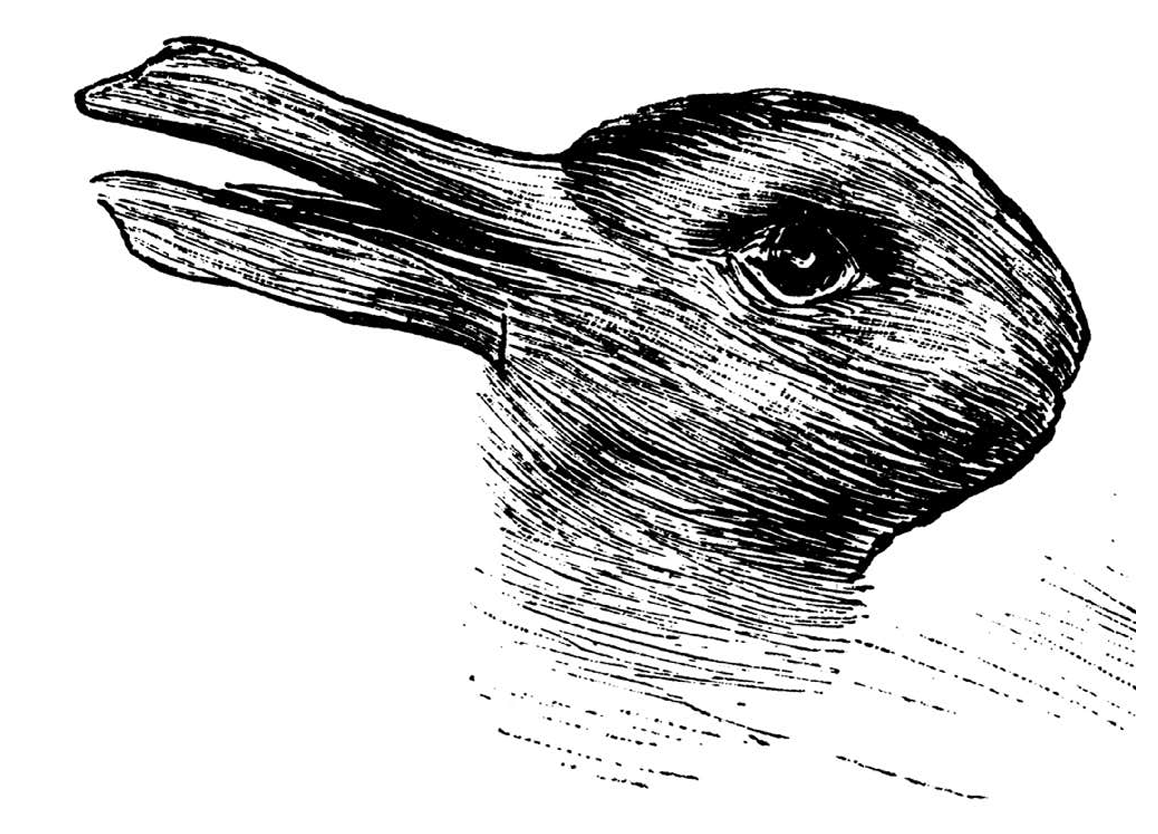
\includegraphics[keepaspectratio]{C:/Users/peakh/Documents/GitHub/Notes_Git/AI-Rosseta/Rosseta_Notes/Books/How to Live/attachments/Pasted image 20250413110648.png}}

这是鸭子还是兔子?\\
不,这是鸭子和兔子。

\pandocbounded{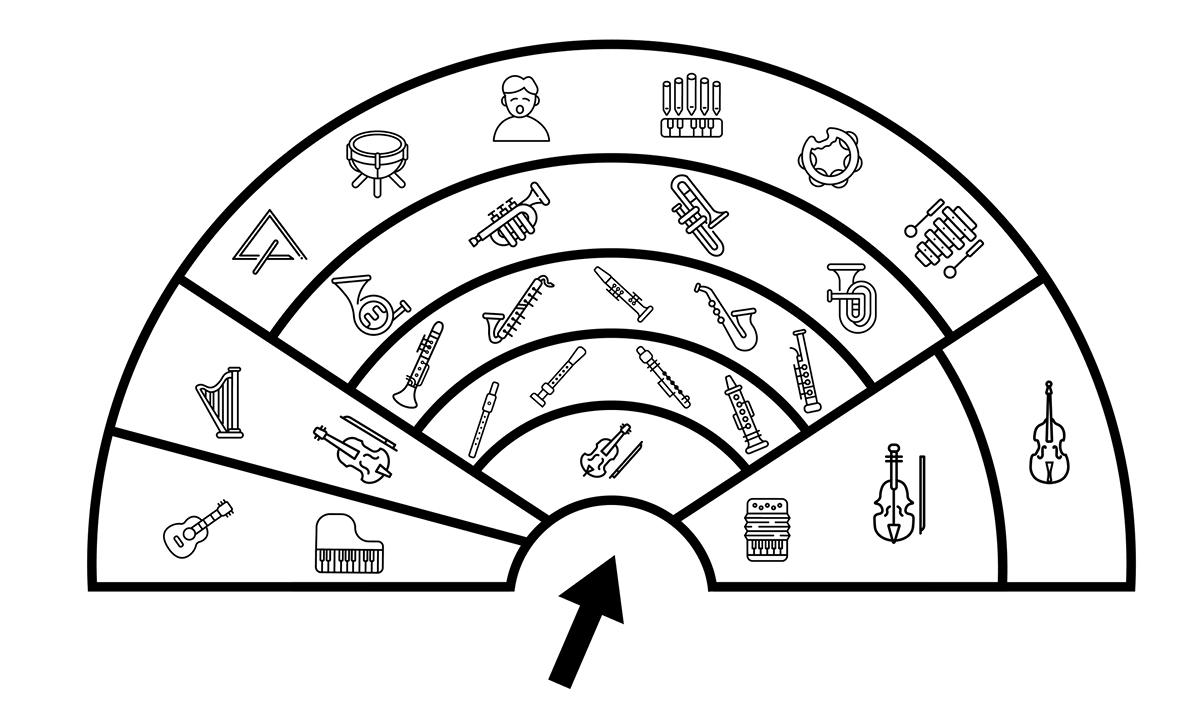
\includegraphics[keepaspectratio]{C:/Users/peakh/Documents/GitHub/Notes_Git/AI-Rosseta/Rosseta_Notes/Books/How to Live/attachments/Pasted image 20250413110712.png}}\\
这是一场交响乐。\\
你是作曲家,也是指挥家。

\subsubsection{\texorpdfstring{关于作者
}{关于作者 }}\label{ux5173ux4e8eux4f5cux8005}

\begin{quote}
\begin{itemize}
\item
  如果你想了解更多关于我或我的作品,请访问
  \href{https://sive.rs}{sive.rs}。一切都在那里。 有任何问题,请访问
  \href{https://sive.rs/contact}{sive.rs/contact} 给我发送邮件。 ------
  Derek
\end{itemize}
\end{quote}

\pandocbounded{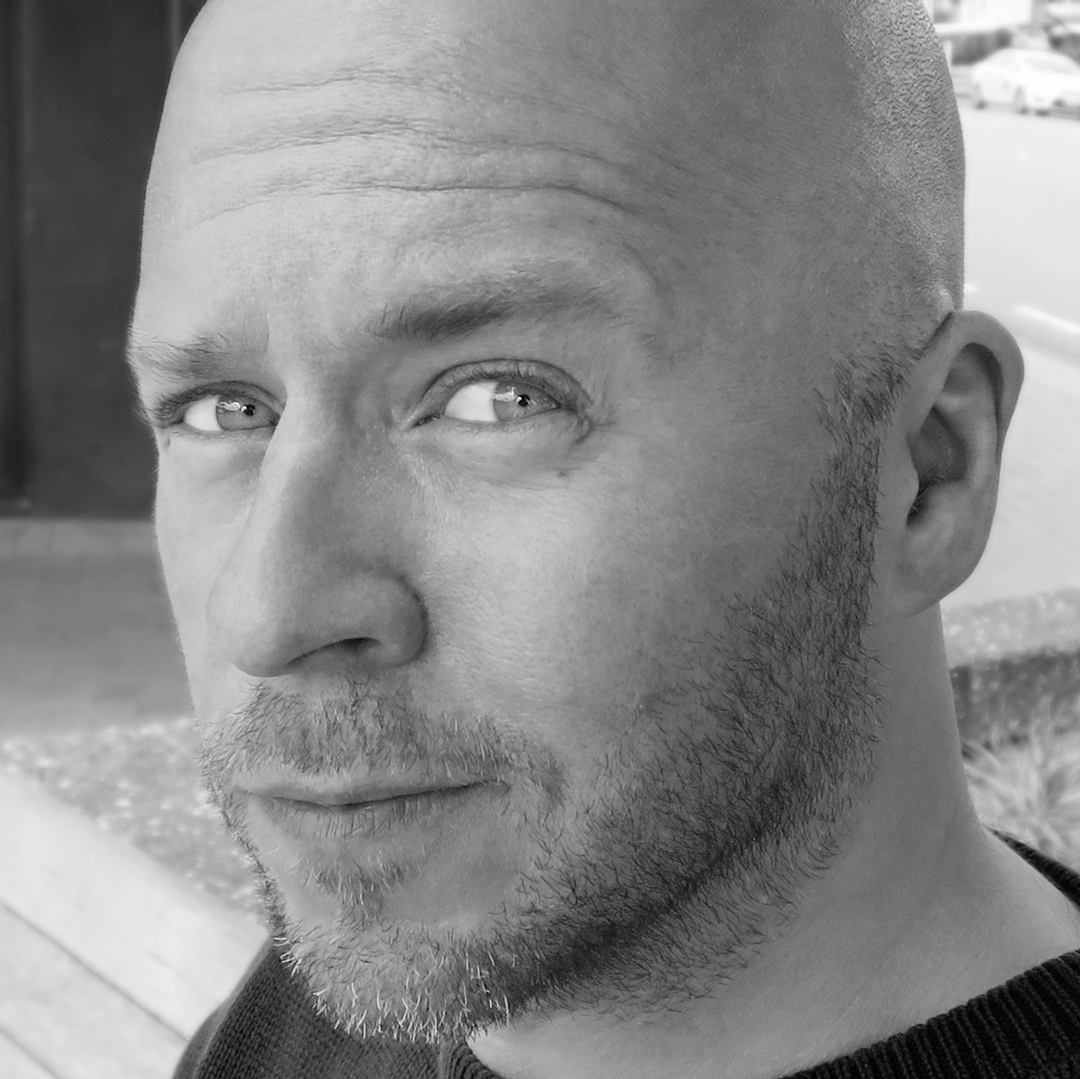
\includegraphics[keepaspectratio]{C:/Users/peakh/Documents/GitHub/Notes_Git/AI-Rosseta/Rosseta_Notes/Books/How to Live/attachments/Pasted image 20250413111156.png}}

\end{document}
